\documentclass[twoside]{report}

%%%%%%%%%%%%%%%%%%%%%%%%%%%%%%%%%
% PACKAGE IMPORTS
%%%%%%%%%%%%%%%%%%%%%%%%%%%%%%%%%


\usepackage[tmargin=2cm,rmargin=1in,lmargin=1in,margin=0.85in,bmargin=2cm,footskip=.2in]{geometry}
\usepackage{amsmath,amsfonts,amsthm,amssymb,mathtools}
\usepackage[varbb]{newpxmath}
\usepackage{xfrac}
\usepackage[makeroom]{cancel}
\usepackage{mathtools}
\usepackage{bookmark}
\usepackage{enumitem}
\usepackage{hyperref,theoremref}
\hypersetup{
	pdftitle={Assignment},
	colorlinks=true, linkcolor=violet,
	bookmarksnumbered=true,
	bookmarksopen=true
}
\usepackage[most,many,breakable]{tcolorbox}
\usepackage{xcolor}
\usepackage{varwidth}
\usepackage{varwidth}
\usepackage{etoolbox}
%\usepackage{authblk}
\usepackage{nameref}
\usepackage{multicol,array}
\usepackage{tikz-cd}
\usepackage[ruled,vlined,linesnumbered]{algorithm2e}
\usepackage{comment} % enables the use of multi-line comments (\ifx \fi) 
\usepackage{import}
\usepackage{xifthen}
\usepackage{pdfpages}
\usepackage{transparent}
\usepackage{afterpage}

\newcommand\mycommfont[1]{\footnotesize\ttfamily\textcolor{violet}{#1}}
\SetCommentSty{mycommfont}
\newcommand{\incfig}[1]{%
    \def\svgwidth{\columnwidth}
    \import{./figures/}{#1.pdf_tex}
}

\usepackage{tikzsymbols}
\renewcommand\qedsymbol{$\Laughey$}


%\usepackage{import}
%\usepackage{xifthen}
%\usepackage{pdfpages}
%\usepackage{transparent}

%%%%%%%%%%%%%%%%%%%%%%%%%%%%%%
% TEX LIVE PACKAGES
%%%%%%%%%%%%%%%%%%%%%%%%%%%%%%

\usepackage[T1]{fontenc}
\usepackage{anyfontsize}

%%%%%%%%%%%%%%%%%%%%%%%%%%%%%%
% BLANK PAGE
%%%%%%%%%%%%%%%%%%%%%%%%%%%%%%

\newcommand\blankpage{%
    \null
    \thispagestyle{empty}%
    \addtocounter{page}{-1}%
    \newpage
}

%%%%%%%%%%%%%%%%%%%%%%%%%%%%%%
% SELF MADE COLORS
%%%%%%%%%%%%%%%%%%%%%%%%%%%%%%



\definecolor{myg}{RGB}{56, 140, 70}
\definecolor{myb}{RGB}{45, 111, 177}
\definecolor{myr}{RGB}{199, 68, 64}
\definecolor{mytheorembg}{HTML}{F2F2F9}
\definecolor{mytheoremfr}{HTML}{00007B}
\definecolor{mylenmabg}{HTML}{FFFAF8}
\definecolor{mylenmafr}{HTML}{983b0f}
\definecolor{mypropbg}{HTML}{f2fbfc}
\definecolor{mypropfr}{HTML}{191971}
\definecolor{myexamplebg}{HTML}{F2FBF8}
\definecolor{myexamplefr}{HTML}{88D6D1}
\definecolor{myexampleti}{HTML}{2A7F7F}
\definecolor{mydefinitbg}{HTML}{E5E5FF}
\definecolor{mydefinitfr}{HTML}{3F3FA3}
\definecolor{notesred}{RGB}{0,162,0}
\definecolor{myp}{RGB}{197, 92, 212}
\definecolor{mygr}{HTML}{2C3338}
\definecolor{myred}{RGB}{127,0,0}
\definecolor{myyellow}{RGB}{169,121,69}
\definecolor{myexercisebg}{HTML}{F2FBF8}
\definecolor{myexercisefg}{HTML}{88D6D1}


%%%%%%%%%%%%%%%%%%%%%%%%%%%%
% TCOLORBOX SETUPS
%%%%%%%%%%%%%%%%%%%%%%%%%%%%

\setlength{\parindent}{1cm}
%================================
% THEOREM BOX
%================================

\tcbuselibrary{theorems,skins,hooks}
\newtcbtheorem[number within=section]{Theorem}{Teorema}
{%
	enhanced,
	breakable,
	colback = mytheorembg,
	frame hidden,
	boxrule = 0sp,
	borderline west = {2pt}{0pt}{mytheoremfr},
	sharp corners,
	detach title,
	before upper = \tcbtitle\par\smallskip,
	coltitle = mytheoremfr,
	fonttitle = \bfseries\sffamily,
	description font = \mdseries,
	separator sign none,
	segmentation style={solid, mytheoremfr},
}
{th}

\tcbuselibrary{theorems,skins,hooks}
\newtcbtheorem[number within=chapter]{theorem}{Theorem}
{%
	enhanced,
	breakable,
	colback = mytheorembg,
	frame hidden,
	boxrule = 0sp,
	borderline west = {2pt}{0pt}{mytheoremfr},
	sharp corners,
	detach title,
	before upper = \tcbtitle\par\smallskip,
	coltitle = mytheoremfr,
	fonttitle = \bfseries\sffamily,
	description font = \mdseries,
	separator sign none,
	segmentation style={solid, mytheoremfr},
}
{th}


\tcbuselibrary{theorems,skins,hooks}
\newtcolorbox{Theoremcon}
{%
	enhanced
	,breakable
	,colback = mytheorembg
	,frame hidden
	,boxrule = 0sp
	,borderline west = {2pt}{0pt}{mytheoremfr}
	,sharp corners
	,description font = \mdseries
	,separator sign none
}

%================================
% Corollery
%================================
\tcbuselibrary{theorems,skins,hooks}
\newtcbtheorem[number within=section]{Corollary}{Corollario}
{%
	enhanced
	,breakable
	,colback = myp!10
	,frame hidden
	,boxrule = 0sp
	,borderline west = {2pt}{0pt}{myp!85!black}
	,sharp corners
	,detach title
	,before upper = \tcbtitle\par\smallskip
	,coltitle = myp!85!black
	,fonttitle = \bfseries\sffamily
	,description font = \mdseries
	,separator sign none
	,segmentation style={solid, myp!85!black}
}
{th}
\tcbuselibrary{theorems,skins,hooks}
\newtcbtheorem[number within=chapter]{corollary}{Corollary}
{%
	enhanced
	,breakable
	,colback = myp!10
	,frame hidden
	,boxrule = 0sp
	,borderline west = {2pt}{0pt}{myp!85!black}
	,sharp corners
	,detach title
	,before upper = \tcbtitle\par\smallskip
	,coltitle = myp!85!black
	,fonttitle = \bfseries\sffamily
	,description font = \mdseries
	,separator sign none
	,segmentation style={solid, myp!85!black}
}
{th}


%================================
% LENMA
%================================

\tcbuselibrary{theorems,skins,hooks}
\newtcbtheorem[number within=section]{Lenma}{Lenma}
{%
	enhanced,
	breakable,
	colback = mylenmabg,
	frame hidden,
	boxrule = 0sp,
	borderline west = {2pt}{0pt}{mylenmafr},
	sharp corners,
	detach title,
	before upper = \tcbtitle\par\smallskip,
	coltitle = mylenmafr,
	fonttitle = \bfseries\sffamily,
	description font = \mdseries,
	separator sign none,
	segmentation style={solid, mylenmafr},
}
{th}

\tcbuselibrary{theorems,skins,hooks}
\newtcbtheorem[number within=chapter]{lenma}{Lenma}
{%
	enhanced,
	breakable,
	colback = mylenmabg,
	frame hidden,
	boxrule = 0sp,
	borderline west = {2pt}{0pt}{mylenmafr},
	sharp corners,
	detach title,
	before upper = \tcbtitle\par\smallskip,
	coltitle = mylenmafr,
	fonttitle = \bfseries\sffamily,
	description font = \mdseries,
	separator sign none,
	segmentation style={solid, mylenmafr},
}
{th}


%================================
% PROPOSITION
%================================

\tcbuselibrary{theorems,skins,hooks}
\newtcbtheorem[number within=section]{Prop}{Proposition}
{%
	enhanced,
	breakable,
	colback = mypropbg,
	frame hidden,
	boxrule = 0sp,
	borderline west = {2pt}{0pt}{mypropfr},
	sharp corners,
	detach title,
	before upper = \tcbtitle\par\smallskip,
	coltitle = mypropfr,
	fonttitle = \bfseries\sffamily,
	description font = \mdseries,
	separator sign none,
	segmentation style={solid, mypropfr},
}
{th}

\tcbuselibrary{theorems,skins,hooks}
\newtcbtheorem[number within=chapter]{prop}{Proposition}
{%
	enhanced,
	breakable,
	colback = mypropbg,
	frame hidden,
	boxrule = 0sp,
	borderline west = {2pt}{0pt}{mypropfr},
	sharp corners,
	detach title,
	before upper = \tcbtitle\par\smallskip,
	coltitle = mypropfr,
	fonttitle = \bfseries\sffamily,
	description font = \mdseries,
	separator sign none,
	segmentation style={solid, mypropfr},
}
{th}


%================================
% CLAIM
%================================

\tcbuselibrary{theorems,skins,hooks}
\newtcbtheorem[number within=section]{claim}{Claim}
{%
	enhanced
	,breakable
	,colback = myg!10
	,frame hidden
	,boxrule = 0sp
	,borderline west = {2pt}{0pt}{myg}
	,sharp corners
	,detach title
	,before upper = \tcbtitle\par\smallskip
	,coltitle = myg!85!black
	,fonttitle = \bfseries\sffamily
	,description font = \mdseries
	,separator sign none
	,segmentation style={solid, myg!85!black}
}
{th}



%================================
% Exercise
%================================

\tcbuselibrary{theorems,skins,hooks}
\newtcbtheorem[number within=section]{Exercise}{Exercise}
{%
	enhanced,
	breakable,
	colback = myexercisebg,
	frame hidden,
	boxrule = 0sp,
	borderline west = {2pt}{0pt}{myexercisefg},
	sharp corners,
	detach title,
	before upper = \tcbtitle\par\smallskip,
	coltitle = myexercisefg,
	fonttitle = \bfseries\sffamily,
	description font = \mdseries,
	separator sign none,
	segmentation style={solid, myexercisefg},
}
{th}

\tcbuselibrary{theorems,skins,hooks}
\newtcbtheorem[number within=chapter]{exercise}{Exercise}
{%
	enhanced,
	breakable,
	colback = myexercisebg,
	frame hidden,
	boxrule = 0sp,
	borderline west = {2pt}{0pt}{myexercisefg},
	sharp corners,
	detach title,
	before upper = \tcbtitle\par\smallskip,
	coltitle = myexercisefg,
	fonttitle = \bfseries\sffamily,
	description font = \mdseries,
	separator sign none,
	segmentation style={solid, myexercisefg},
}
{th}

%================================
% EXAMPLE BOX
%================================

\newtcbtheorem[number within=section]{Example}{Esempio}
{%
	colback = myexamplebg
	,breakable
	,colframe = myexamplefr
	,coltitle = myexampleti
	,boxrule = 1pt
	,sharp corners
	,detach title
	,before upper=\tcbtitle\par\smallskip
	,fonttitle = \bfseries
	,description font = \mdseries
	,separator sign none
	,description delimiters parenthesis
}
{ex}

\newtcbtheorem[number within=chapter]{example}{Esempio}
{%
	colback = myexamplebg
	,breakable
	,colframe = myexamplefr
	,coltitle = myexampleti
	,boxrule = 1pt
	,sharp corners
	,detach title
	,before upper=\tcbtitle\par\smallskip
	,fonttitle = \bfseries
	,description font = \mdseries
	,separator sign none
	,description delimiters parenthesis
}
{ex}

%================================
% DEFINITION BOX
%================================

\newtcbtheorem[number within=section]{Definizione}{Definizione}{enhanced,
	before skip=2mm,after skip=2mm, colback=red!5,colframe=red!80!black,boxrule=0.5mm,
	attach boxed title to top left={xshift=1cm,yshift*=1mm-\tcboxedtitleheight}, varwidth boxed title*=-3cm,
	boxed title style={frame code={
					\path[fill=tcbcolback]
					([yshift=-1mm,xshift=-1mm]frame.north west)
					arc[start angle=0,end angle=180,radius=1mm]
					([yshift=-1mm,xshift=1mm]frame.north east)
					arc[start angle=180,end angle=0,radius=1mm];
					\path[left color=tcbcolback!60!black,right color=tcbcolback!60!black,
						middle color=tcbcolback!80!black]
					([xshift=-2mm]frame.north west) -- ([xshift=2mm]frame.north east)
					[rounded corners=1mm]-- ([xshift=1mm,yshift=-1mm]frame.north east)
					-- (frame.south east) -- (frame.south west)
					-- ([xshift=-1mm,yshift=-1mm]frame.north west)
					[sharp corners]-- cycle;
				},interior engine=empty,
		},
	fonttitle=\bfseries,
	title={#2},#1}{def}
\newtcbtheorem[number within=chapter]{definizione}{Definizione}{enhanced,
	before skip=2mm,after skip=2mm, colback=red!5,colframe=red!80!black,boxrule=0.5mm,
	attach boxed title to top left={xshift=1cm,yshift*=1mm-\tcboxedtitleheight}, varwidth boxed title*=-3cm,
	boxed title style={frame code={
					\path[fill=tcbcolback]
					([yshift=-1mm,xshift=-1mm]frame.north west)
					arc[start angle=0,end angle=180,radius=1mm]
					([yshift=-1mm,xshift=1mm]frame.north east)
					arc[start angle=180,end angle=0,radius=1mm];
					\path[left color=tcbcolback!60!black,right color=tcbcolback!60!black,
						middle color=tcbcolback!80!black]
					([xshift=-2mm]frame.north west) -- ([xshift=2mm]frame.north east)
					[rounded corners=1mm]-- ([xshift=1mm,yshift=-1mm]frame.north east)
					-- (frame.south east) -- (frame.south west)
					-- ([xshift=-1mm,yshift=-1mm]frame.north west)
					[sharp corners]-- cycle;
				},interior engine=empty,
		},
	fonttitle=\bfseries,
	title={#2},#1}{def}



%================================
% Solution BOX
%================================

\makeatletter
\newtcbtheorem{question}{Question}{enhanced,
	breakable,
	colback=white,
	colframe=myb!80!black,
	attach boxed title to top left={yshift*=-\tcboxedtitleheight},
	fonttitle=\bfseries,
	title={#2},
	boxed title size=title,
	boxed title style={%
			sharp corners,
			rounded corners=northwest,
			colback=tcbcolframe,
			boxrule=0pt,
		},
	underlay boxed title={%
			\path[fill=tcbcolframe] (title.south west)--(title.south east)
			to[out=0, in=180] ([xshift=5mm]title.east)--
			(title.center-|frame.east)
			[rounded corners=\kvtcb@arc] |-
			(frame.north) -| cycle;
		},
	#1
}{def}
\makeatother

%================================
% SOLUTION BOX
%================================

\makeatletter
\newtcolorbox{solution}{enhanced,
	breakable,
	colback=white,
	colframe=myg!80!black,
	attach boxed title to top left={yshift*=-\tcboxedtitleheight},
	title=Solution,
	boxed title size=title,
	boxed title style={%
			sharp corners,
			rounded corners=northwest,
			colback=tcbcolframe,
			boxrule=0pt,
		},
	underlay boxed title={%
			\path[fill=tcbcolframe] (title.south west)--(title.south east)
			to[out=0, in=180] ([xshift=5mm]title.east)--
			(title.center-|frame.east)
			[rounded corners=\kvtcb@arc] |-
			(frame.north) -| cycle;
		},
}
\makeatother

%================================
% Question BOX
%================================

\makeatletter
\newtcbtheorem{qstion}{Question}{enhanced,
	breakable,
	colback=white,
	colframe=mygr,
	attach boxed title to top left={yshift*=-\tcboxedtitleheight},
	fonttitle=\bfseries,
	title={#2},
	boxed title size=title,
	boxed title style={%
			sharp corners,
			rounded corners=northwest,
			colback=tcbcolframe,
			boxrule=0pt,
		},
	underlay boxed title={%
			\path[fill=tcbcolframe] (title.south west)--(title.south east)
			to[out=0, in=180] ([xshift=5mm]title.east)--
			(title.center-|frame.east)
			[rounded corners=\kvtcb@arc] |-
			(frame.north) -| cycle;
		},
	#1
}{def}
\makeatother

\newtcbtheorem[number within=chapter]{wconc}{Wrong Concept}{
	breakable,
	enhanced,
	colback=white,
	colframe=myr,
	arc=0pt,
	outer arc=0pt,
	fonttitle=\bfseries\sffamily\large,
	colbacktitle=myr,
	attach boxed title to top left={},
	boxed title style={
			enhanced,
			skin=enhancedfirst jigsaw,
			arc=3pt,
			bottom=0pt,
			interior style={fill=myr}
		},
	#1
}{def}



%================================
% NOTE BOX
%================================

\usetikzlibrary{arrows,calc,shadows.blur}
\tcbuselibrary{skins}
\newtcolorbox{note}[1][]{%
	enhanced jigsaw,
	colback=gray!20!white,%
	colframe=gray!80!black,
	size=small,
	boxrule=1pt,
	title=\textbf{Note:-},
	halign title=flush center,
	coltitle=black,
	breakable,
	drop shadow=black!50!white,
	attach boxed title to top left={xshift=1cm,yshift=-\tcboxedtitleheight/2,yshifttext=-\tcboxedtitleheight/2},
	minipage boxed title=1.5cm,
	boxed title style={%
			colback=white,
			size=fbox,
			boxrule=1pt,
			boxsep=2pt,
			underlay={%
					\coordinate (dotA) at ($(interior.west) + (-0.5pt,0)$);
					\coordinate (dotB) at ($(interior.east) + (0.5pt,0)$);
					\begin{scope}
						\clip (interior.north west) rectangle ([xshift=3ex]interior.east);
						\filldraw [white, blur shadow={shadow opacity=60, shadow yshift=-.75ex}, rounded corners=2pt] (interior.north west) rectangle (interior.south east);
					\end{scope}
					\begin{scope}[gray!80!black]
						\fill (dotA) circle (2pt);
						\fill (dotB) circle (2pt);
					\end{scope}
				},
		},
	#1,
}

%%%%%%%%%%%%%%%%%%%%%%%%%%%%%%
% SELF MADE COMMANDS
%%%%%%%%%%%%%%%%%%%%%%%%%%%%%%


\newcommand{\thm}[2]{\begin{Theorem}{#1}{}#2\end{Theorem}}
\newcommand{\cor}[2]{\begin{Corollary}{#1}{}#2\end{Corollary}}
\newcommand{\mlenma}[2]{\begin{Lenma}{#1}{}#2\end{Lenma}}
\newcommand{\mprop}[2]{\begin{Prop}{#1}{}#2\end{Prop}}
\newcommand{\clm}[3]{\begin{claim}{#1}{#2}#3\end{claim}}
\newcommand{\wc}[2]{\begin{wconc}{#1}{}\setlength{\parindent}{1cm}#2\end{wconc}}
\newcommand{\thmcon}[1]{\begin{Theoremcon}{#1}\end{Theoremcon}}
\newcommand{\ex}[2]{\begin{Example}{#1}{}#2\end{Example}}
\newcommand{\dfn}[2]{\begin{Definizione}[colbacktitle=red!75!black]{#1}{}#2\end{Definizione}}
\newcommand{\dfnc}[2]{\begin{definizione}[colbacktitle=red!75!black]{#1}{}#2\end{definizione}}
\newcommand{\qs}[2]{\begin{question}{#1}{}#2\end{question}}
\newcommand{\pf}[2]{\begin{myproof}[#1]#2\end{myproof}}
\newcommand{\nt}[1]{\begin{note}#1\end{note}}

\newcommand*\circled[1]{\tikz[baseline=(char.base)]{
		\node[shape=circle,draw,inner sep=1pt] (char) {#1};}}
\newcommand\getcurrentref[1]{%
	\ifnumequal{\value{#1}}{0}
	{??}
	{\the\value{#1}}%
}
\newcommand{\getCurrentSectionNumber}{\getcurrentref{section}}
\newenvironment{myproof}[1][\proofname]{%
	\proof[\bfseries #1: ]%
}{\endproof}

\newcommand{\mclm}[2]{\begin{myclaim}[#1]#2\end{myclaim}}
\newenvironment{myclaim}[1][\claimname]{\proof[\bfseries #1: ]}{}

\newcounter{mylabelcounter}

\makeatletter
\newcommand{\setword}[2]{%
	\phantomsection
	#1\def\@currentlabel{\unexpanded{#1}}\label{#2}%
}
\makeatother




\tikzset{
	symbol/.style={
			draw=none,
			every to/.append style={
					edge node={node [sloped, allow upside down, auto=false]{$#1$}}}
		}
}


% deliminators
\DeclarePairedDelimiter{\abs}{\lvert}{\rvert}
\DeclarePairedDelimiter{\norm}{\lVert}{\rVert}

\DeclarePairedDelimiter{\ceil}{\lceil}{\rceil}
\DeclarePairedDelimiter{\floor}{\lfloor}{\rfloor}
\DeclarePairedDelimiter{\round}{\lfloor}{\rceil}

\newsavebox\diffdbox
\newcommand{\slantedromand}{{\mathpalette\makesl{d}}}
\newcommand{\makesl}[2]{%
\begingroup
\sbox{\diffdbox}{$\mathsurround=0pt#1\mathrm{#2}$}%
\pdfsave
\pdfsetmatrix{1 0 0.2 1}%
\rlap{\usebox{\diffdbox}}%
\pdfrestore
\hskip\wd\diffdbox
\endgroup
}
\newcommand{\dd}[1][]{\ensuremath{\mathop{}\!\ifstrempty{#1}{%
\slantedromand\@ifnextchar^{\hspace{0.2ex}}{\hspace{0.1ex}}}%
{\slantedromand\hspace{0.2ex}^{#1}}}}
\ProvideDocumentCommand\dv{o m g}{%
  \ensuremath{%
    \IfValueTF{#3}{%
      \IfNoValueTF{#1}{%
        \frac{\dd #2}{\dd #3}%
      }{%
        \frac{\dd^{#1} #2}{\dd #3^{#1}}%
      }%
    }{%
      \IfNoValueTF{#1}{%
        \frac{\dd}{\dd #2}%
      }{%
        \frac{\dd^{#1}}{\dd #2^{#1}}%
      }%
    }%
  }%
}
\providecommand*{\pdv}[3][]{\frac{\partial^{#1}#2}{\partial#3^{#1}}}
%  - others
\DeclareMathOperator{\Lap}{\mathcal{L}}
\DeclareMathOperator{\Var}{Var} % varience
\DeclareMathOperator{\Cov}{Cov} % covarience
\DeclareMathOperator{\E}{E} % expected

% Since the amsthm package isn't loaded

% I prefer the slanted \leq
\let\oldleq\leq % save them in case they're every wanted
\let\oldgeq\geq
\renewcommand{\leq}{\leqslant}
\renewcommand{\geq}{\geqslant}

% % redefine matrix env to allow for alignment, use r as default
% \renewcommand*\env@matrix[1][r]{\hskip -\arraycolsep
%     \let\@ifnextchar\new@ifnextchar
%     \array{*\c@MaxMatrixCols #1}}


%\usepackage{framed}
%\usepackage{titletoc}
%\usepackage{etoolbox}
%\usepackage{lmodern}


%\patchcmd{\tableofcontents}{\contentsname}{\sffamily\contentsname}{}{}

%\renewenvironment{leftbar}
%{\def\FrameCommand{\hspace{6em}%
%		{\color{myyellow}\vrule width 2pt depth 6pt}\hspace{1em}}%
%	\MakeFramed{\parshape 1 0cm \dimexpr\textwidth-6em\relax\FrameRestore}\vskip2pt%
%}
%{\endMakeFramed}

%\titlecontents{chapter}
%[0em]{\vspace*{2\baselineskip}}
%{\parbox{4.5em}{%
%		\hfill\Huge\sffamily\bfseries\color{myred}\thecontentspage}%
%	\vspace*{-2.3\baselineskip}\leftbar\textsc{\small\chaptername~\thecontentslabel}\\\sffamily}
%{}{\endleftbar}
%\titlecontents{section}
%[8.4em]
%{\sffamily\contentslabel{3em}}{}{}
%{\hspace{0.5em}\nobreak\itshape\color{myred}\contentspage}
%\titlecontents{subsection}
%[8.4em]
%{\sffamily\contentslabel{3em}}{}{}  
%{\hspace{0.5em}\nobreak\itshape\color{myred}\contentspage}



%%%%%%%%%%%%%%%%%%%%%%%%%%%%%%%%%%%%%%%%%%%
% TABLE OF CONTENTS
%%%%%%%%%%%%%%%%%%%%%%%%%%%%%%%%%%%%%%%%%%%

\usepackage{tikz}
\definecolor{doc}{RGB}{0,60,110}
\usepackage{titletoc}
\contentsmargin{0cm}
\titlecontents{chapter}[3.7pc]
{\addvspace{30pt}%
	\begin{tikzpicture}[remember picture, overlay]%
		\draw[fill=violet,draw=violet] (-7.3,-.1) rectangle (-0.5,.5);%
		\pgftext[left,x=-3.7cm,y=0.2cm]{\color{white}\Large\sc\bfseries Capitolo\ \thecontentslabel};%
	\end{tikzpicture}\color{violet}\large\sc\bfseries}%
{}
{}
{\;\titlerule\;\large\sc\bfseries Pagina \thecontentspage
	\begin{tikzpicture}[remember picture, overlay]
		\draw[fill=violet,draw=violet] (2pt,0) rectangle (4,0.1pt);
	\end{tikzpicture}}%
\titlecontents{section}[3.7pc]
{\addvspace{2pt}}
{\contentslabel[\thecontentslabel]{2pc}}
{}
{\hfill\small \thecontentspage}
[]
\titlecontents*{subsection}[3.7pc]
{\addvspace{-1pt}\small}
{}
{}
{\ --- \small\thecontentspage}
[ \textbullet\ ][]

\makeatletter
\renewcommand{\chaptername}{Capitolo}
\renewcommand{\tableofcontents}{%
	\chapter*{%
	  \vspace*{-20\p@}%
	  \begin{tikzpicture}[remember picture, overlay]%
		  \pgftext[right,x=15cm,y=0.2cm]{\color{violet}\Huge\sc\bfseries \contentsname};%
		  \draw[fill=violet,draw=violet] (13,-.75) rectangle (20,1);%
		  \clip (13,-.75) rectangle (20,1);
		  \pgftext[right,x=15cm,y=0.2cm]{\color{white}\Huge\sc\bfseries \contentsname};%
	  \end{tikzpicture}}%
	\@starttoc{toc}}
\makeatother

%%%%%%%%%%%%%%%%%%%%%%%%%%%%%%%%%%%%%%%%%%%
% HYPERLINK
%%%%%%%%%%%%%%%%%%%%%%%%%%%%%%%%%%%%%%%%%%%

\hypersetup{
    colorlinks,
    citecolor=black,
    filecolor=black,
    linkcolor=black,
    urlcolor=black
}
%From M275 "Topology" at SJSU
\newcommand{\id}{\mathrm{id}}
\newcommand{\taking}[1]{\xrightarrow{#1}}
\newcommand{\inv}{^{-1}}

%From M170 "Introduction to Graph Theory" at SJSU
\DeclareMathOperator{\diam}{diam}
\DeclareMathOperator{\ord}{ord}
\newcommand{\defeq}{\overset{\mathrm{def}}{=}}

%From the USAMO .tex files
\newcommand{\ts}{\textsuperscript}
\newcommand{\dg}{^\circ}
\newcommand{\ii}{\item}

% % From Math 55 and Math 145 at Harvard
% \newenvironment{subproof}[1][Proof]{%
% \begin{proof}[#1] \renewcommand{\qedsymbol}{$\blacksquare$}}%
% {\end{proof}}

\newcommand{\ac}{\Leftrightarrow_\alpha}
\newcommand{\br}{\rightarrow_\beta}
\newcommand{\er}{\rightarrow_\eta}
\newcommand{\liff}{\leftrightarrow}
\newcommand{\lthen}{\rightarrow}
\newcommand{\opname}{\operatorname}
\newcommand{\surjto}{\twoheadrightarrow}
\newcommand{\injto}{\hookrightarrow}
\newcommand{\On}{\mathrm{On}} % ordinals
\DeclareMathOperator{\img}{im} % Image
\DeclareMathOperator{\Img}{Im} % Image
\DeclareMathOperator{\coker}{coker} % Cokernel
\DeclareMathOperator{\Coker}{Coker} % Cokernel
\DeclareMathOperator{\Ker}{Ker} % Kernel
\DeclareMathOperator{\rank}{rank}
\DeclareMathOperator{\Spec}{Spec} % spectrum
\DeclareMathOperator{\Tr}{Tr} % trace
\DeclareMathOperator{\pr}{pr} % projection
\DeclareMathOperator{\ext}{ext} % extension
\DeclareMathOperator{\pred}{pred} % predecessor
\DeclareMathOperator{\dom}{dom} % domain
\DeclareMathOperator{\ran}{ran} % range
\DeclareMathOperator{\Hom}{Hom} % homomorphism
\DeclareMathOperator{\Mor}{Mor} % morphisms
\DeclareMathOperator{\End}{End} % endomorphism

\newcommand{\eps}{\epsilon}
\newcommand{\veps}{\varepsilon}
\newcommand{\ol}{\overline}
\newcommand{\ul}{\underline}
\newcommand{\wt}{\widetilde}
\newcommand{\wh}{\widehat}
\newcommand{\vocab}[1]{\textbf{\color{blue} #1}}
\providecommand{\half}{\frac{1}{2}}
\newcommand{\dang}{\measuredangle} %% Directed angle
\newcommand{\ray}[1]{\overrightarrow{#1}}
\newcommand{\seg}[1]{\overline{#1}}
\newcommand{\arc}[1]{\wideparen{#1}}
\DeclareMathOperator{\cis}{cis}
\DeclareMathOperator*{\lcm}{lcm}
\DeclareMathOperator*{\argmin}{arg min}
\DeclareMathOperator*{\argmax}{arg max}
\newcommand{\cycsum}{\sum_{\mathrm{cyc}}}
\newcommand{\symsum}{\sum_{\mathrm{sym}}}
\newcommand{\cycprod}{\prod_{\mathrm{cyc}}}
\newcommand{\symprod}{\prod_{\mathrm{sym}}}
\newcommand{\Qed}{\begin{flushright}\qed\end{flushright}}
\newcommand{\parinn}{\setlength{\parindent}{1cm}}
\newcommand{\parinf}{\setlength{\parindent}{0cm}}
% \newcommand{\norm}{\|\cdot\|}
\newcommand{\inorm}{\norm_{\infty}}
\newcommand{\opensets}{\{V_{\alpha}\}_{\alpha\in I}}
\newcommand{\oset}{V_{\alpha}}
\newcommand{\opset}[1]{V_{\alpha_{#1}}}
\newcommand{\lub}{\text{lub}}
\newcommand{\del}[2]{\frac{\partial #1}{\partial #2}}
\newcommand{\Del}[3]{\frac{\partial^{#1} #2}{\partial^{#1} #3}}
\newcommand{\deld}[2]{\dfrac{\partial #1}{\partial #2}}
\newcommand{\Deld}[3]{\dfrac{\partial^{#1} #2}{\partial^{#1} #3}}
\newcommand{\lm}{\lambda}
\newcommand{\uin}{\mathbin{\rotatebox[origin=c]{90}{$\in$}}}
\newcommand{\usubset}{\mathbin{\rotatebox[origin=c]{90}{$\subset$}}}
\newcommand{\lt}{\left}
\newcommand{\rt}{\right}
\newcommand{\bs}[1]{\boldsymbol{#1}}
\newcommand{\exs}{\exists}
\newcommand{\st}{\strut}
\newcommand{\dps}[1]{\displaystyle{#1}}

\newcommand{\sol}{\setlength{\parindent}{0cm}\textbf{\textit{Solution:}}\setlength{\parindent}{1cm} }
\newcommand{\solve}[1]{\setlength{\parindent}{0cm}\textbf{\textit{Solution: }}\setlength{\parindent}{1cm}#1 \Qed}
% Things Lie
\newcommand{\kb}{\mathfrak b}
\newcommand{\kg}{\mathfrak g}
\newcommand{\kh}{\mathfrak h}
\newcommand{\kn}{\mathfrak n}
\newcommand{\ku}{\mathfrak u}
\newcommand{\kz}{\mathfrak z}
\DeclareMathOperator{\Ext}{Ext} % Ext functor
\DeclareMathOperator{\Tor}{Tor} % Tor functor
\newcommand{\gl}{\opname{\mathfrak{gl}}} % frak gl group
\renewcommand{\sl}{\opname{\mathfrak{sl}}} % frak sl group chktex 6

% More script letters etc.
\newcommand{\SA}{\mathcal A}
\newcommand{\SB}{\mathcal B}
\newcommand{\SC}{\mathcal C}
\newcommand{\SF}{\mathcal F}
\newcommand{\SG}{\mathcal G}
\newcommand{\SH}{\mathcal H}
\newcommand{\OO}{\mathcal O}

\newcommand{\SCA}{\mathscr A}
\newcommand{\SCB}{\mathscr B}
\newcommand{\SCC}{\mathscr C}
\newcommand{\SCD}{\mathscr D}
\newcommand{\SCE}{\mathscr E}
\newcommand{\SCF}{\mathscr F}
\newcommand{\SCG}{\mathscr G}
\newcommand{\SCH}{\mathscr H}

% Mathfrak primes
\newcommand{\km}{\mathfrak m}
\newcommand{\kp}{\mathfrak p}
\newcommand{\kq}{\mathfrak q}

% number sets
\newcommand{\RR}[1][]{\ensuremath{\ifstrempty{#1}{\mathbb{R}}{\mathbb{R}^{#1}}}}
\newcommand{\NN}[1][]{\ensuremath{\ifstrempty{#1}{\mathbb{N}}{\mathbb{N}^{#1}}}}
\newcommand{\ZZ}[1][]{\ensuremath{\ifstrempty{#1}{\mathbb{Z}}{\mathbb{Z}^{#1}}}}
\newcommand{\QQ}[1][]{\ensuremath{\ifstrempty{#1}{\mathbb{Q}}{\mathbb{Q}^{#1}}}}
\newcommand{\CC}[1][]{\ensuremath{\ifstrempty{#1}{\mathbb{C}}{\mathbb{C}^{#1}}}}
\newcommand{\PP}[1][]{\ensuremath{\ifstrempty{#1}{\mathbb{P}}{\mathbb{P}^{#1}}}}
\newcommand{\HH}[1][]{\ensuremath{\ifstrempty{#1}{\mathbb{H}}{\mathbb{H}^{#1}}}}
\newcommand{\FF}[1][]{\ensuremath{\ifstrempty{#1}{\mathbb{F}}{\mathbb{F}^{#1}}}}
% expected value
\newcommand{\EE}{\ensuremath{\mathbb{E}}}
\newcommand{\charin}{\text{ char }}
\DeclareMathOperator{\sign}{sign}
\DeclareMathOperator{\Aut}{Aut}
\DeclareMathOperator{\Inn}{Inn}
\DeclareMathOperator{\Syl}{Syl}
\DeclareMathOperator{\Gal}{Gal}
\DeclareMathOperator{\GL}{GL} % General linear group
\DeclareMathOperator{\SL}{SL} % Special linear group

%---------------------------------------
% BlackBoard Math Fonts :-
%---------------------------------------

%Captital Letters
\newcommand{\bbA}{\mathbb{A}}	\newcommand{\bbB}{\mathbb{B}}
\newcommand{\bbC}{\mathbb{C}}	\newcommand{\bbD}{\mathbb{D}}
\newcommand{\bbE}{\mathbb{E}}	\newcommand{\bbF}{\mathbb{F}}
\newcommand{\bbG}{\mathbb{G}}	\newcommand{\bbH}{\mathbb{H}}
\newcommand{\bbI}{\mathbb{I}}	\newcommand{\bbJ}{\mathbb{J}}
\newcommand{\bbK}{\mathbb{K}}	\newcommand{\bbL}{\mathbb{L}}
\newcommand{\bbM}{\mathbb{M}}	\newcommand{\bbN}{\mathbb{N}}
\newcommand{\bbO}{\mathbb{O}}	\newcommand{\bbP}{\mathbb{P}}
\newcommand{\bbQ}{\mathbb{Q}}	\newcommand{\bbR}{\mathbb{R}}
\newcommand{\bbS}{\mathbb{S}}	\newcommand{\bbT}{\mathbb{T}}
\newcommand{\bbU}{\mathbb{U}}	\newcommand{\bbV}{\mathbb{V}}
\newcommand{\bbW}{\mathbb{W}}	\newcommand{\bbX}{\mathbb{X}}
\newcommand{\bbY}{\mathbb{Y}}	\newcommand{\bbZ}{\mathbb{Z}}

%---------------------------------------
% MathCal Fonts :-
%---------------------------------------

%Captital Letters
\newcommand{\mcA}{\mathcal{A}}	\newcommand{\mcB}{\mathcal{B}}
\newcommand{\mcC}{\mathcal{C}}	\newcommand{\mcD}{\mathcal{D}}
\newcommand{\mcE}{\mathcal{E}}	\newcommand{\mcF}{\mathcal{F}}
\newcommand{\mcG}{\mathcal{G}}	\newcommand{\mcH}{\mathcal{H}}
\newcommand{\mcI}{\mathcal{I}}	\newcommand{\mcJ}{\mathcal{J}}
\newcommand{\mcK}{\mathcal{K}}	\newcommand{\mcL}{\mathcal{L}}
\newcommand{\mcM}{\mathcal{M}}	\newcommand{\mcN}{\mathcal{N}}
\newcommand{\mcO}{\mathcal{O}}	\newcommand{\mcP}{\mathcal{P}}
\newcommand{\mcQ}{\mathcal{Q}}	\newcommand{\mcR}{\mathcal{R}}
\newcommand{\mcS}{\mathcal{S}}	\newcommand{\mcT}{\mathcal{T}}
\newcommand{\mcU}{\mathcal{U}}	\newcommand{\mcV}{\mathcal{V}}
\newcommand{\mcW}{\mathcal{W}}	\newcommand{\mcX}{\mathcal{X}}
\newcommand{\mcY}{\mathcal{Y}}	\newcommand{\mcZ}{\mathcal{Z}}


%---------------------------------------
% Bold Math Fonts :-
%---------------------------------------

%Captital Letters
\newcommand{\bmA}{\boldsymbol{A}}	\newcommand{\bmB}{\boldsymbol{B}}
\newcommand{\bmC}{\boldsymbol{C}}	\newcommand{\bmD}{\boldsymbol{D}}
\newcommand{\bmE}{\boldsymbol{E}}	\newcommand{\bmF}{\boldsymbol{F}}
\newcommand{\bmG}{\boldsymbol{G}}	\newcommand{\bmH}{\boldsymbol{H}}
\newcommand{\bmI}{\boldsymbol{I}}	\newcommand{\bmJ}{\boldsymbol{J}}
\newcommand{\bmK}{\boldsymbol{K}}	\newcommand{\bmL}{\boldsymbol{L}}
\newcommand{\bmM}{\boldsymbol{M}}	\newcommand{\bmN}{\boldsymbol{N}}
\newcommand{\bmO}{\boldsymbol{O}}	\newcommand{\bmP}{\boldsymbol{P}}
\newcommand{\bmQ}{\boldsymbol{Q}}	\newcommand{\bmR}{\boldsymbol{R}}
\newcommand{\bmS}{\boldsymbol{S}}	\newcommand{\bmT}{\boldsymbol{T}}
\newcommand{\bmU}{\boldsymbol{U}}	\newcommand{\bmV}{\boldsymbol{V}}
\newcommand{\bmW}{\boldsymbol{W}}	\newcommand{\bmX}{\boldsymbol{X}}
\newcommand{\bmY}{\boldsymbol{Y}}	\newcommand{\bmZ}{\boldsymbol{Z}}
%Small Letters
\newcommand{\bma}{\boldsymbol{a}}	\newcommand{\bmb}{\boldsymbol{b}}
\newcommand{\bmc}{\boldsymbol{c}}	\newcommand{\bmd}{\boldsymbol{d}}
\newcommand{\bme}{\boldsymbol{e}}	\newcommand{\bmf}{\boldsymbol{f}}
\newcommand{\bmg}{\boldsymbol{g}}	\newcommand{\bmh}{\boldsymbol{h}}
\newcommand{\bmi}{\boldsymbol{i}}	\newcommand{\bmj}{\boldsymbol{j}}
\newcommand{\bmk}{\boldsymbol{k}}	\newcommand{\bml}{\boldsymbol{l}}
\newcommand{\bmm}{\boldsymbol{m}}	\newcommand{\bmn}{\boldsymbol{n}}
\newcommand{\bmo}{\boldsymbol{o}}	\newcommand{\bmp}{\boldsymbol{p}}
\newcommand{\bmq}{\boldsymbol{q}}	\newcommand{\bmr}{\boldsymbol{r}}
\newcommand{\bms}{\boldsymbol{s}}	\newcommand{\bmt}{\boldsymbol{t}}
\newcommand{\bmu}{\boldsymbol{u}}	\newcommand{\bmv}{\boldsymbol{v}}
\newcommand{\bmw}{\boldsymbol{w}}	\newcommand{\bmx}{\boldsymbol{x}}
\newcommand{\bmy}{\boldsymbol{y}}	\newcommand{\bmz}{\boldsymbol{z}}

%---------------------------------------
% Scr Math Fonts :-
%---------------------------------------

\newcommand{\sA}{{\mathscr{A}}}   \newcommand{\sB}{{\mathscr{B}}}
\newcommand{\sC}{{\mathscr{C}}}   \newcommand{\sD}{{\mathscr{D}}}
\newcommand{\sE}{{\mathscr{E}}}   \newcommand{\sF}{{\mathscr{F}}}
\newcommand{\sG}{{\mathscr{G}}}   \newcommand{\sH}{{\mathscr{H}}}
\newcommand{\sI}{{\mathscr{I}}}   \newcommand{\sJ}{{\mathscr{J}}}
\newcommand{\sK}{{\mathscr{K}}}   \newcommand{\sL}{{\mathscr{L}}}
\newcommand{\sM}{{\mathscr{M}}}   \newcommand{\sN}{{\mathscr{N}}}
\newcommand{\sO}{{\mathscr{O}}}   \newcommand{\sP}{{\mathscr{P}}}
\newcommand{\sQ}{{\mathscr{Q}}}   \newcommand{\sR}{{\mathscr{R}}}
\newcommand{\sS}{{\mathscr{S}}}   \newcommand{\sT}{{\mathscr{T}}}
\newcommand{\sU}{{\mathscr{U}}}   \newcommand{\sV}{{\mathscr{V}}}
\newcommand{\sW}{{\mathscr{W}}}   \newcommand{\sX}{{\mathscr{X}}}
\newcommand{\sY}{{\mathscr{Y}}}   \newcommand{\sZ}{{\mathscr{Z}}}


%---------------------------------------
% Math Fraktur Font
%---------------------------------------

%Captital Letters
\newcommand{\mfA}{\mathfrak{A}}	\newcommand{\mfB}{\mathfrak{B}}
\newcommand{\mfC}{\mathfrak{C}}	\newcommand{\mfD}{\mathfrak{D}}
\newcommand{\mfE}{\mathfrak{E}}	\newcommand{\mfF}{\mathfrak{F}}
\newcommand{\mfG}{\mathfrak{G}}	\newcommand{\mfH}{\mathfrak{H}}
\newcommand{\mfI}{\mathfrak{I}}	\newcommand{\mfJ}{\mathfrak{J}}
\newcommand{\mfK}{\mathfrak{K}}	\newcommand{\mfL}{\mathfrak{L}}
\newcommand{\mfM}{\mathfrak{M}}	\newcommand{\mfN}{\mathfrak{N}}
\newcommand{\mfO}{\mathfrak{O}}	\newcommand{\mfP}{\mathfrak{P}}
\newcommand{\mfQ}{\mathfrak{Q}}	\newcommand{\mfR}{\mathfrak{R}}
\newcommand{\mfS}{\mathfrak{S}}	\newcommand{\mfT}{\mathfrak{T}}
\newcommand{\mfU}{\mathfrak{U}}	\newcommand{\mfV}{\mathfrak{V}}
\newcommand{\mfW}{\mathfrak{W}}	\newcommand{\mfX}{\mathfrak{X}}
\newcommand{\mfY}{\mathfrak{Y}}	\newcommand{\mfZ}{\mathfrak{Z}}
%Small Letters
\newcommand{\mfa}{\mathfrak{a}}	\newcommand{\mfb}{\mathfrak{b}}
\newcommand{\mfc}{\mathfrak{c}}	\newcommand{\mfd}{\mathfrak{d}}
\newcommand{\mfe}{\mathfrak{e}}	\newcommand{\mff}{\mathfrak{f}}
\newcommand{\mfg}{\mathfrak{g}}	\newcommand{\mfh}{\mathfrak{h}}
\newcommand{\mfi}{\mathfrak{i}}	\newcommand{\mfj}{\mathfrak{j}}
\newcommand{\mfk}{\mathfrak{k}}	\newcommand{\mfl}{\mathfrak{l}}
\newcommand{\mfm}{\mathfrak{m}}	\newcommand{\mfn}{\mathfrak{n}}
\newcommand{\mfo}{\mathfrak{o}}	\newcommand{\mfp}{\mathfrak{p}}
\newcommand{\mfq}{\mathfrak{q}}	\newcommand{\mfr}{\mathfrak{r}}
\newcommand{\mfs}{\mathfrak{s}}	\newcommand{\mft}{\mathfrak{t}}
\newcommand{\mfu}{\mathfrak{u}}	\newcommand{\mfv}{\mathfrak{v}}
\newcommand{\mfw}{\mathfrak{w}}	\newcommand{\mfx}{\mathfrak{x}}
\newcommand{\mfy}{\mathfrak{y}}	\newcommand{\mfz}{\mathfrak{z}}

\renewcommand{\contentsname}{Indice}
\RequirePackage[times]{quotchap}
\definecolor{chaptergrey}{rgb}{0.7,0,0}
\usepackage{fancyhdr}



\def\layout{2}  


\title{
    \Huge{\textcolor{1}{\textbf{Storia dell'Informatica - Seconda Parte}}\\
    \textcolor{4}{\hrulefill} \\
    \textcolor{6}{\textbf{Appunti}}}
}
\author{\huge{Luca Barra}}
\date{\textbf{Anno accademico 2023/2024}
\begin{figure}[h]
    \centering
    
\includegraphics[scale=0.5]{images/unito_logo.png}
\end{figure}
}

\begin{document}

\maketitle

\newpage% or \cleardoublepage
% \pdfbookmark[<level>]{<title>}{<dest>}
\pdfbookmark[section]{\contentsname}{toc}
\afterpage{\blankpage}
\pagenumbering{Roman}
\tableofcontents
\cleardoublepage\pagenumbering{arabic}

%%%%%%%%%%%%%%%%%%%%%%%%%%%%%%
% EXPERIMENT
%%%%%%%%%%%%%%%%%%%%%%%%%%%%%%
\pagestyle{fancy}

\ifnum\layout=2 
    \fancyhf{}      
    \renewcommand{\headrulewidth}{0pt}
    \renewcommand{\chaptermark}[1]{{\markboth{#1}{}}}

    \fancyhead[LE]{\nouppercase{\textbf{\textcolor{chaptergrey}{\chaptername}}~ \thechapter~ |~ \leftmark}}
    \fancyhead[RO]{\nouppercase{ \rightmark}}
    \fancyfoot[LE,RO]{\thepage}
    \fancypagestyle{plain}{         
    \fancyhf{}
    \fancyfoot[LE,RO]{\thepage}}    
 \else          
    \renewcommand{\headrulewidth}{0pt}
    \fancyhf{}                  
    \textcolor{red}{\fancyhead[C]{\nouppercase{ \leftmark}}}
    \fancyfoot[C]{\thepage}
\fi

\chapter{Premessa}

\section{Licenza}

Questi appunti sono rilasciati sotto licenza Creative Commons Attribuzione 4.0 Internazionale (per maggiori
informazioni consultare il link: \href{https://creativecommons.org/version4/}{https://creativecommons.org/version4/}). Sono basati sulle slides del corso "Storia dell'Informatica" del prof. Felice Cardone.
\begin{center}
    
\includegraphics[width=0.5\textwidth]{images/cc.png}
\end{center}

\section{Formato utilizzato}

In questi appunti vengono utilizzati molti \fancyglitter{box}. Questa è una semplice 
rassegna che ne spiega l'utilizzo:

\subsubsection{Box di "Concetto sbagliato":}

\wc{Testo del concetto sbagliato}{
    Testo contente il concetto giusto.
}

\subsubsection{Box di "Corollario":}

\cor{Nome del corollario}{
    Testo del corollario. Per corollario si intende una definizione minore,
    legata a un'altra definizione.
}

\subsubsection{Box di "Definizione":}

\dfn{Nome delle definizione}{
    Testo della definizione.
}

\subsubsection{Box di "Domanda":}

\qs{}{
    Testo della domanda. Le domande sono spesso utilizzate per far riflettere
    sulle definizioni o sui concetti.
}

\subsubsection{Box di "Esempio":}

\ex{Nome dell'esempio}{
    Testo dell'esempio. Gli esempi sono tratti dalle slides del corso.
}

\subsubsection{Box di "Note":}

\nt{
    Testo della nota. Le note sono spesso utilizzate per chiarire concetti
    o per dare informazioni aggiuntive.
}

\subsubsection{Box di "Meta-nota":}

\clm{}{}{Testo della meta-nota. Le meta-note utilizzate 
    com note più personali per fornire riflessioni e motivazioni al 
    perchè si sta facendo ciò che si sta facendo. Vengono usate per 
    simulare lo stile espositivo del prof. Cardone che spazia in poco tempo 
    su molti argomenti.
    Possono essere scollegate direttamente dal contesto in cui si trovano e ai fini degli appunti
    possono essere tranquillamente ignorate.
}

\subsubsection{Box di "Teorema":}

\thm{Nome del teorema}{
    Testo del teorema. 
}
\afterpage{\blankpage}

\definecolor{chaptergrey}{rgb}{0,0.7,0}
\ifnum\layout=2 
    \fancyhf{}      
    \renewcommand{\headrulewidth}{0pt}
    \renewcommand{\chaptermark}[1]{\markboth{#1}{}}

    \fancyhead[LE]{\nouppercase{\textbf{\textcolor{chaptergrey}{\chaptername}}~ \thechapter~ |~ \leftmark}}
    \fancyhead[RO]{\nouppercase{ \rightmark}}
    \fancyfoot[LE,RO]{\thepage}
    \fancypagestyle{plain}{         
    \fancyhf{}
    \fancyfoot[LE,RO]{\thepage}}    
 \else          
    \renewcommand{\headrulewidth}{0pt}
    \fancyhf{}                  
    \fancyhead[C]{\nouppercase{ \leftmark}}
    \fancyfoot[C]{\thepage}
\fi
\chapter{Dalla semiotica a von Neumann}

Il corso si divide in una serie di sezioni:
\begin{itemize}
    \item [$\Rightarrow$] Macchine mai esistite (Knowledge
    Navigator, Dynabook, Memex): poichè la storia dell'informatica
    è una storia di idee, di pionieri e di visionari;
    \item [$\Rightarrow$] Il modo di organizzare i testi in rapporto all'inondazione 
    informativa: workstation di Otlet (non realizzata), the mother of all
    demos (Doug Engelbart, 1968), gli ipertesti di Ted Nelson, libraries
    of the future;
    \item [$\Rightarrow$] La cybernetica: originata da Norbert Wiener, ci si concentra sugli
    aspetti matematici della neurofisiologia che portarono al modello formale di
    neurone (McCulloch e Pitts, 1943) utilizzato da von Neumann per la
    definizione della sua architettura di calcolatore;
    \item [$\Rightarrow$] Gli hippies e la controcultura: si parla di come la controcultura 
    abbia influenzato la nascita dell'informatica;
    \item [$\Rightarrow$] La semiotica: si parte in ordine cronologico dalla preistoria, passando per Lullo fino
    a Leibniz, per arrivare ai sistemi formali.
\end{itemize}

\section{La preistoria dell'informatica}

\qs{}{Perchè studiare cosi indietro nel tempo?}

\paragraph{Risposta:} perchè si vuole caratterizzare il
concetto di calcolo e si vogliono comprendere le abilità cognitive
su cui tale concetto si basa.

\subsubsection{}

Circa 110.000 anni fa si ha, in Cina, il primo esempio di astrazione con degli \newfancyglitter{ossi intagliati}. Essa è la produzione consapevole di una traccia relativamente stabile. Successivamente, intorno al 8000 a. C., sono stati usati dei \newfancyglitter{gettoni} in argilla. Presumibilmente questa è la nascita simultanea della scrittura e del calcolo. I gettoni vennero affiancati dalle \newfancyglitter{tavolette d'argilla}, modellate usando dei calchi (come un rudimentale libro contabile).

\paragraph{I gettoni:}

\begin{itemize}
    \item [$\Rightarrow$] Favoriscono la raccolta di dati;
    \item [$\Rightarrow$] Sono immediati da comprendere;
    \item [$\Rightarrow$] Permettono le operazioni aritmetiche come manipolazioni concrete.
\end{itemize}

Un ulteriore fenomeno è quello delle \newfancyglitter{bolle} che contengono dei gettoni. Venivano usate come registrazione di un contratto quando un proprietario di bestiame dava in affitto la sua mandria per la transumanza.

Oltre agli strumenti d'argilla vennero usati dei \newfancyglitter{bastoncini di legno} che venivano divisi in due metà: una ricevuta e un titolo di credito. Il titolo di credito si chiamava \newfancyglitter{stock} (da qui il termine "stock market") e la ricevuta si chiamava stub.

\subsection{Semiotica}

Nei meccanismi illustrati nella sezione precedente i segni hanno un ruolo importante. 

\dfn{Semiotica}{La \newfancyglitter{semiotica} è la scienza che studia i linguaggi e i segni che li costituiscono.}

\cor{Il linguaggio}{In ogni linguaggio sono presenti tre componenti:

\begin{itemize}
    \item [$\Rightarrow$] Chi produce i segni (studiati dalla pragmatica);
    \item [$\Rightarrow$] I segni prodotti (studiati dalla sintassi);
    \item [$\Rightarrow$] Il significato dei segni (studiati dalla semantica).
\end{itemize}
}

\paragraph{La semiotica è direttamente collegata all'informatica (computer semiotics):}

\begin{itemize}
    \item [$\Rightarrow$] Un computer è spesso utilizzato per generare, trasformare e visualizzare segni (il PC come medium);
    \item [$\Rightarrow$] Un computer viene programmato utilizzando un linguaggio.
\end{itemize}

\subsection{Kenneth Iverson e Raimondo Lullo}

\newfancyglitter{Kenneth Iverson} fu un importate semiotico e fu il fondatore del linguaggio esoterico APL, che nacque come linguaggio logico. APL influenzo molti linguaggi funzionali, come Haskell, e il paradigma di parallelismo.

\begin{center}
    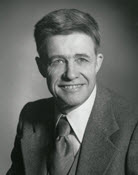
\includegraphics[scale = 1]{images/iverson.jpg}
\end{center}

\subsubsection{}

Un altro personaggio importante fu Raimondo Lullo, un filosofo, teologo e missionario catalano. Egli fu il primo a proporre un sistema di combinazione di segni per ottenere nuove conoscenze. Il suo sistema era basato su un insieme di simboli che rappresentavano le nozioni e le relazioni tra di esse. Questo sistema era chiamato \newfancyglitter{Ars Magna}.
Oltre a ciò si occupò di \newfancyglitter{logica combinatoria} nella sua opera \newfancyglitter{Ars Combinatoria}.

\section{Leibniz}

Nasce a Lipsia il 21 Giugno 1646, si laurea in Giurisprudenza nel 1666.
I suoi primi scritti sono finalizzati al conseguimento di titoli accademici. Importante in
questo periodo è la Dissertatio de Arte Combinatoria del 1666.
Negli anni immediatamente successivi alla laurea diventa consigliere dell’Elettore di
Magonza ed assume diversi incarichi politici.

\begin{center}
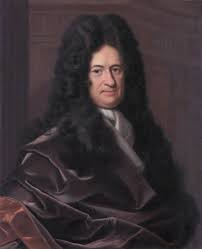
\includegraphics[scale = 0.7]{images/Leibniz.jpg}
\end{center}

Nel 1672 viene inviato a Parigi in missione diplomatica, per distogliere Luigi XIV dalla
progettata invasione dell’Olanda ed invogliarlo invece alla conquista dell’Egitto.
Fallita la missione, ottiene il permesso di fermarsi a Parigi (e Londra), dove rimane per 4
anni (marzo 1672-ottobre 1676) avendo la possibilità di conoscere la matematica e la
fisica più avanzate. Nel 1676 scopre il calcolo infinitesimale (che verrà pubblicato solo ne 1684), già
introdotto da Newton indipendentemente 10 anni prima. Nel 1705 inizierà tra i due una
polemica che finirà solo con la morte di Leibniz.
Nello stesso anno torna ad Hannover come bibliotecario presso il Duca di Hannover.

Tra il 1685 e il 1694: migliora la scatola di Pascal (\newfancyglitter{pascalina}) per l’addizione e la sottrazione per realizzare
anche la moltiplicazione e la divisione (e l’estrazione di radice). La macchina, che opera
mediante pulegge e ruote dentate, è conservata nella biblioteca di Hannover.

\subsection{L'origine del bit}

Leibniz fece un parallelismo tra i simboli dello yin e dello yang e i numeri binari.
Le linee piene potevano essere associate al 1, mentre le linee vuote al 0.
Così facendo si ottiene un sistema di numerazione binario.

\begin{center}
    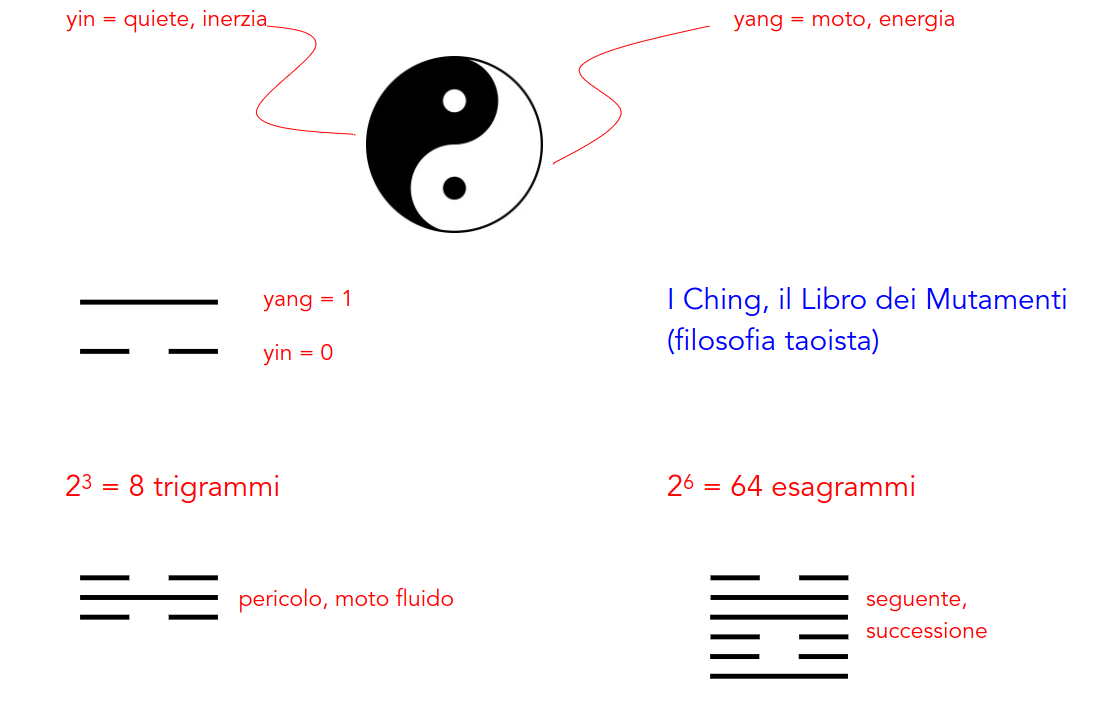
\includegraphics[scale = 0.3]{images/Origine bit.png}
\end{center}

\pagebreak

\ex{L'interpretazione di Leibniz}{
    \begin{center}
        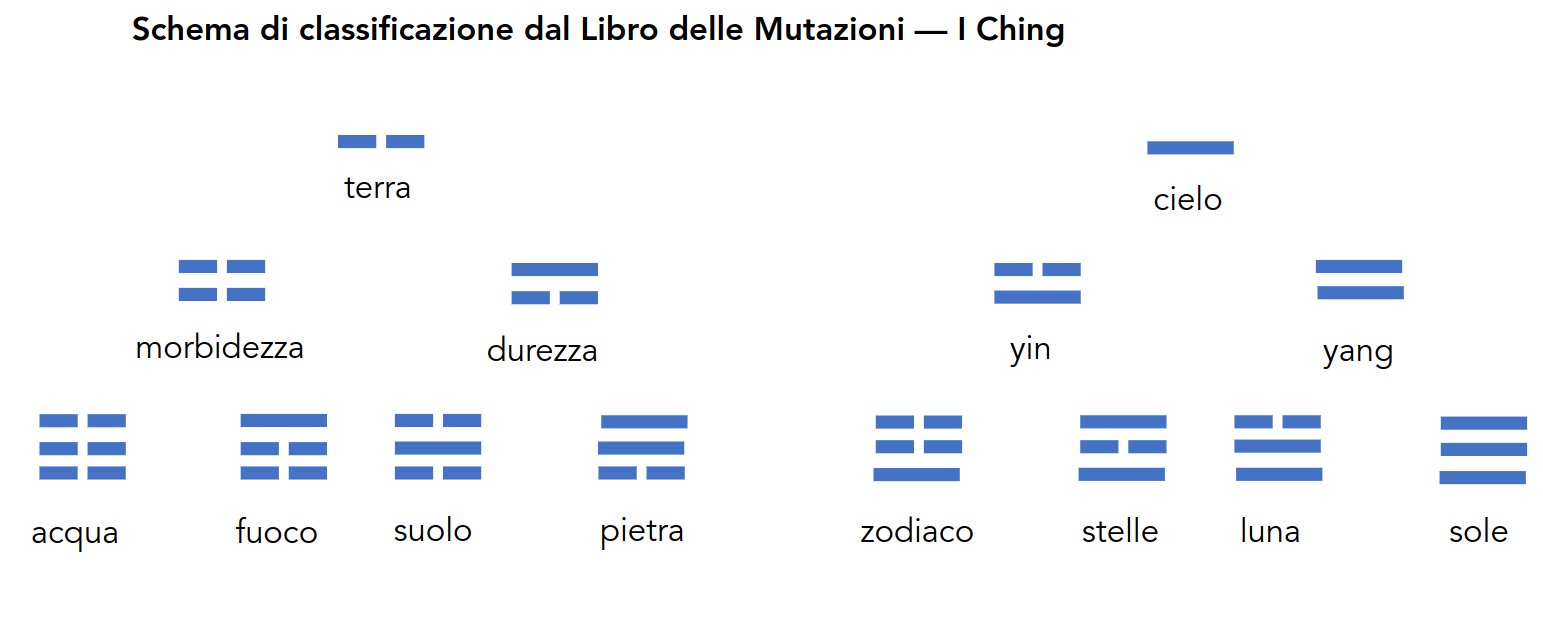
\includegraphics[scale = 0.27]{images/Bit.png}
        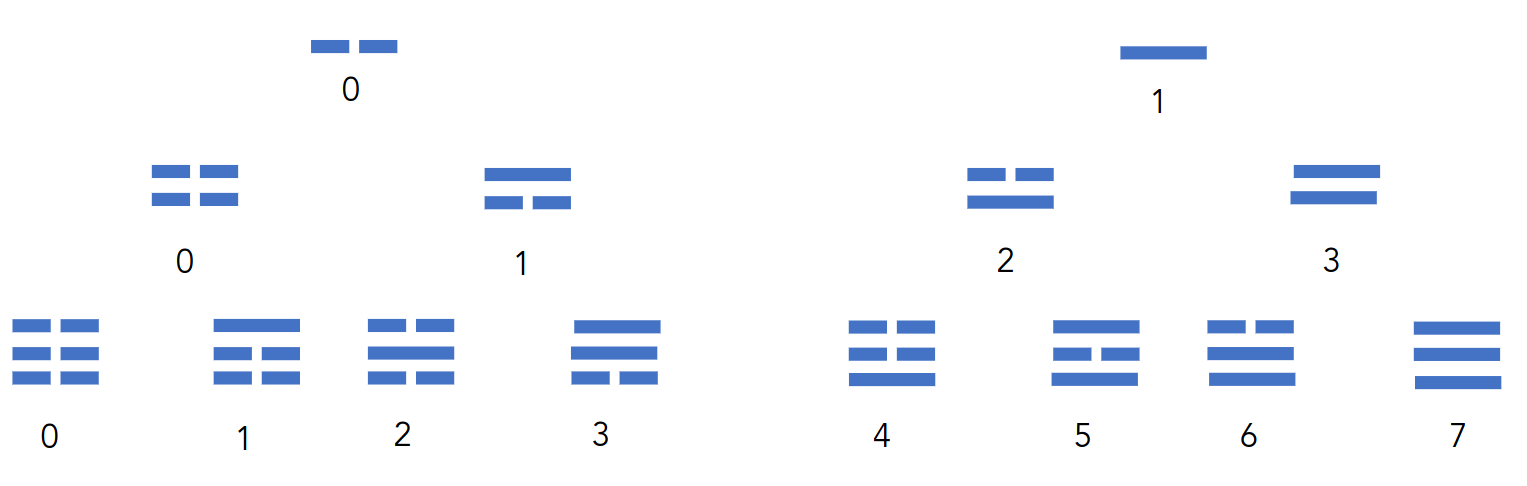
\includegraphics[scale = 0.27]{images/Associazione di Leibniz.png}
    \end{center}
}

\subsection{La caratteristica universale}

La \newfancyglitter{caratteristica universale}, concepita come lingua o scrittura universale, si fonda sui seguenti principi:

\begin{itemize}
    \item [$\Rightarrow$] Le idee sono analizzabili fino a idee semplici (atomiche);
    \item [$\Rightarrow$] Le idee possono essere rappresentate da simboli;
    \item [$\Rightarrow$] Le relazioni tra idee possono essere rappresentate da simboli;
    \item [$\Rightarrow$] Le idee si combinano mediante regole.
\end{itemize}

\dfn{Caratteristica universale}{
La \newfancyglitter{caratteristica universale}\footnote{Ispirata da Lullo e dal "Lullismo", da Atanasio Kircher e da uno scrittore anonimo del 1963.} è un sistema di segni che rappresentano
nozioni e cose, ma non parole. Le connessioni tra i segni rappresentano le relazioni tra le nozioni e le cose.
Il nome di una nozione serve a:
\begin{itemize}
    \item [$\Rightarrow$] Relazionarla con altre nozioni;
    \item [$\Rightarrow$] Relazionarla con lo schema dell'universo;
    \item [$\Rightarrow$] Indicare le esperienze necessarie per la conoscenza.
\end{itemize}
}

\nt{L'apprendimento della lingua universale coincide con l'\fancyglitter{enciclopedia}. }


\subsubsection{Il calculus ratiocinator}

\dfn{Calculus ratiocinator}{Il \newfancyglitter{calculus ratiocinator} è un insieme di tecniche per manipolare i segni della caratteristica universale. Può essere considerato come un \newfancyglitter{sistema formale}. Il frammento XX offre un'idea di questo calcolo: in esso vengono trattati molti assiomi e teoremi come il principio degli indiscernibili, la simmetria, la transitività, etc.}

\subsection{La mereologia del Frammento XX}

\dfn{Mereologia}{
    La \newfancyglitter{mereologia} è la "dottrina delle parti".
}

\dfn{Principio di identità degli indiscernibili}{
    Sono identici i termini che possono essere sostituiti a vicenda
    senza alterare la verità degli enunciati in cui compaiono. Si scrive A = B 
    quando A e B sono identici.
    \begin{itemize}
        \item [$\Rightarrow$] $B + N = L$ significa che B e N compongono L,
        cioè che B è parte di L;
        \item [$\Rightarrow$] $A\leq B$ significa che A è parte di B.
    \end{itemize}
}

\thm{Simmetria}{
    Se $A = B$ allora $B = A$.
}

\thm{Transitività}{
    Se $A = B$ e $B = C$ allora $A = C$.
}

\thm{}{
    Se $A + B = B$ allora $A \leq B$.
}

\thm{}{
    Se $A = B$ allora $A + L = B + L$.
}
\pagebreak
\section{Ulteriori sviluppi}

\subsection{Peano e i numeri naturali}

Peano nacque a Cuneo il 27 agosto 1858. Si laureò in matematica nel 1880 e divenne professore di analisi matematica a Torino nel 1890. Nel 1889 pubblicò i suoi famosi \newfancyglitter{Principi di aritmetica}, in cui formulò un sistema assiomatico per i numeri naturali.

\begin{center}
    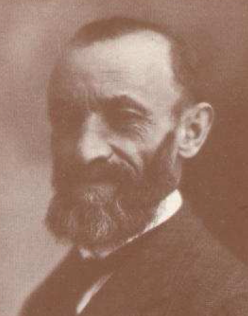
\includegraphics[scale = 0.7]{images/Peano.png}
\end{center}

\dfn{Principi di aritmetica}{
    I \newfancyglitter{Principi di aritmetica} sono un insieme
    di assiomi che definiscono i numeri naturali.
}

\subsection{Hilbert e lo Entscheidungsproblem}

Hilbert fu un matematico tedesco nato a Königsberg il 23 gennaio 1862. Egli fu uno dei più grandi matematici del XX secolo e fu uno dei fondatori della logica matematica.
Nel 1928, insieme ad Ackermann, pubblicò il libro \newfancyglitter{Grundzüge der theoretischen Logik} in cui si venne enunciato il \newfancyglitter{problema della decisione} (
    o \newfancyglitter{Entscheidungsproblem}).

\dfn{Entscheidungsproblem}{
    L'\newfancyglitter{Entscheidungsproblem} è un problema che consiste nel trovare una procedura che consente di decidere la validità di una data espressione logica con un 
    numero finito di operazioni.
}

\pagebreak

\section{La logica matematica}

\nt{Sono trattati più in dettaglio nel corso "Metodi formali dell'Informatica" e, in
misura minore, nel corso di "Linguaggi e paradigmi di programmazione".}

\subsection{Sistemi formali}

\dfn{Sistema formale}{
    In un \newfancyglitter{sistema formale} si definiscono:
    \begin{itemize}
        \item [$\Rightarrow$] \fancyglitter{Oggetti}, che sono tutti i termini costruibili a partire 
        da atomi mediante operazioni;
        \item [$\Rightarrow$] \fancyglitter{Proposizioni}, della forma $P(a_1, ..., a_n)$ dove
        $P$ è un \fancyglitter{predicato} e $a_k$ sono termini;
        \item [$\Rightarrow$] \fancyglitter{Regole di inferenza}, che permettono di dedurre nuove proposizioni.
        La conclusione di una regola di inferenza senza premesse è un'\fancyglitter{assioma}.
    \end{itemize}

    $$\frac{A_1 \:\:\:\:\:\:\:\:\:...\:\:\:\:\:\:\:\:\: A_v}{A}$$
}

\qs{}{Come si usano le regole di inferenza?}

\paragraph{Risposta:} Per costruire derivazioni: 

\begin{figure}[h]
    \centering
    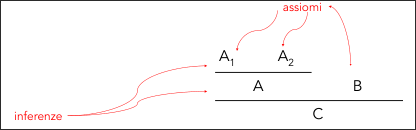
\includegraphics[scale = 0.35]{images/Inferenza.png}
    \caption{Derivazione.}
\end{figure}

\ex{Numeri naturali}{
    \begin{itemize}
        \item [$\Rightarrow$] \fancyglitter{Oggetti}: un atomo 0, un'operazione S, con un solo argomento;
        \item [$\Rightarrow$] \fancyglitter{Proposizioni}: un predicato Num con un solo argomento;
        \item [$\Rightarrow$] \fancyglitter{Regole di inferenza}: $\frac{}{\text{Num\{0\}}}$ e 
        $\frac{\text{Num\{n\}}}{\text{Num\{S(n)\}}}$.
    \end{itemize}
}

\ex{Grammatiche formali}{
    \begin{center}
        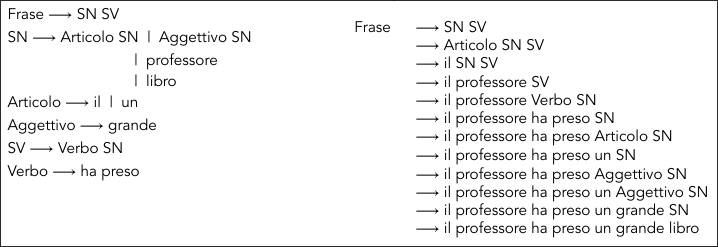
\includegraphics[scale = 0.35]{images/Gram.png}
    \end{center}
}

\subsection{Confronto tra logica e informatica}

\paragraph{Logica:}

\begin{itemize}
    \item [$\Rightarrow$] Si studiano modelli di processi deduttivi;
    \item [$\Rightarrow$] Si studiano modelli di ragionamento;
    \item [$\Rightarrow$] Operatori modali.
\end{itemize}

\paragraph{Informatica:}

\begin{itemize}
    \item [$\Rightarrow$] Si studiano modelli di processi trasformazionali;
    \item [$\Rightarrow$] Si studiano modelli di calcolo (sequenziali, paralleli, distribuiti).
\end{itemize}


\subsection{Kleene e le funzioni ricorsive}

Nel 1981 Stephen Cole Kleene, matematico e logico statunitense,
pubblicò l'articolo "\fancyglitter{Origins of recursive function theory}" in cui
descrisse l'attività di ricerca svolta da alcuni matematici
e logici negli anni '30. In particolare, Kleene descrisse
una serie di lezioni di G\"odel tenute nel 1934 a Princeton
sullo sviluppo di definizioni ricorsive primitive di funzioni 
numeriche. Lo \fancyglitter{schema di ricorsione primitiva} permette di
definire una funzione di numeri naturali f(\textbf{x}, n) a partire da funzioni 
predefinite b(\textbf{x}) e h(\textbf{x}, n, m) mediante lo schema:

$$f(x, 0) = b(x)$$

$$f(x, n + 1) = h(x, n , f(x, n))$$
\subsubsection*{}
Inoltre si ha la composizione:

$$f(x) = h(g_1(x), \cdot\cdot\cdot, g_k(x))$$

\subsubsection*{}

G\"odel usava la nozione di \newfancyglitter{sistema matematico formale} basata
sulla nozione informale di \newfancyglitter{regola costruttiva} la cui
applicazione si basava su una \newfancyglitter{procedura finita} del tipo
necessario per calcolare funzioni definite mediante ricorsioni generali.
\subsubsection{}
Nasce il problema della caratterizzazione delle ricorsioni ammissibili.
Kleene aggiunse un \fancyglitter{operatore di ricerca} non limitato
che dato un predicato P(x, y) restituisce il valore minimo che soddisfa
il predicato. 
Nel 1938, Kleene ammise la possibilità di definire funzioni
parziali.

\section{Curry e la logica combinatoria}

Nel 1927, Haskell Brooks Curry, matematico e logico statunitense,
riscopri la nozione di \fancyglitter{combinatore} (introdotta da
Moses Sch\"onfinkel nel 1920).

\dfn{Combinatore}{
    Un \newfancyglitter{combinatore} è una funzione senza variabili libere.
}

\nt{I sistemi di combinatori attuali usano K e S come combinatori,
perchè sono sufficienti a generare tutti gli altri combinatori.}

\ex{Combinatori}{
    \begin{itemize}
        \item [$\Rightarrow$] K(x, y) = x;
        \item [$\Rightarrow$] S(x, y, z) = x(z)(y(z)).;
        \item [$\Rightarrow$] B(x, y, z) = x(y(z));
        \item [$\Rightarrow$] C(x, y, z) = x(z)(y);
        \item [$\Rightarrow$] W(x, y) = x(y)(y).
        \item [$\Rightarrow$] I(x) = x.
    \end{itemize}
}

\subsubsection*{}

Inoltre riprende anche la possibilità di trattare funzioni a più argomenti
come funzioni a un solo argomento che verrà chiamata \newfancyglitter{curryficazione}.

$$f(x, y) = f'(x)(y)$$

\subsubsection*{}

Nello stesso tempo, Alonzo Church, sviluppa il \newfancyglitter{lambda calcolo}\footnote{Visto approfonditamente nei corsi 
"Metodi formali dell'informatica" e "Linguaggi e paradigmi di programmazione, per cui in questi appunti non andrò
in dettaglio dato che esula gli obiettivi del corso.}.

\dfn{Lambda calcolo}{
    Il \newfancyglitter{lambda calcolo} è un sistema formale per la definizione di funzioni
    intese come regole di corrispondenza. $\lambda x.M$ descrive la regola che assegna
    a un argomento $x$ il valore $M$.
}

\subsection{Paradosso di Russell e combinatori}

$$WS(BWB) = Y = \lambda x.(\lambda z.x(zz)) (\lambda z.x(zz))$$

\nt{Si tratta del combinatore di punto fisso.
Permette di definire funzioni ricorsive.}

\dfn{Paradosso di Russell}{

    $$(\lambda x.(\lambda z.x(zz)) (\lambda z.x(zz))) \neg = 
     (\lambda z.\neg(zz)) (\lambda z.\neg(zz))$$

    In cui $\{z | \neg (z \in z)\} \in \{z | \neg (z \in z)\}$.
    Ciò vuol dire che qualcosa appartiene a se stesso, ma
    non può appartenere a se stesso.

}

\section{L'analisi dei processi di calcolo di Turing}

Nel paragrafo 9 del suo articolo del 1936, Turing introduce
il comportamento di un \fancyglitter{computor}. Lo esemplifica con un
foglio di carta che viene astratto come un "nastro infinito" suddiviso in
caselle (quadratini):
\begin{itemize}
    \item [$\Rightarrow$] Il numero di simboli che si possono stampare è finito,
    perchè se ci fossero infiniti simboli ci si potrebbe confondere\footnote{Un po'
    come il fatto che molti caratteri Unicode non possono essere usati nei
    nomi dei siti web in quanto troppo "simili".};
    \item [$\Rightarrow$] Il comportamento è determinato dallo stato mentale
    e dal simbolo osservato, c'è un limite alla percezione delle caselle per lo stesso
    motivo di prima;
    \item [$\Rightarrow$] Le operazioni sono elementari, cioè non possono essere
    ulteriormente scomposte. Esse consistono in cambiamenti di stato mentale e  
    del simbolo osservato\footnote{Un solo simbolo viene alterato.}.
\end{itemize}

\begin{figure}[h]
    \centering
    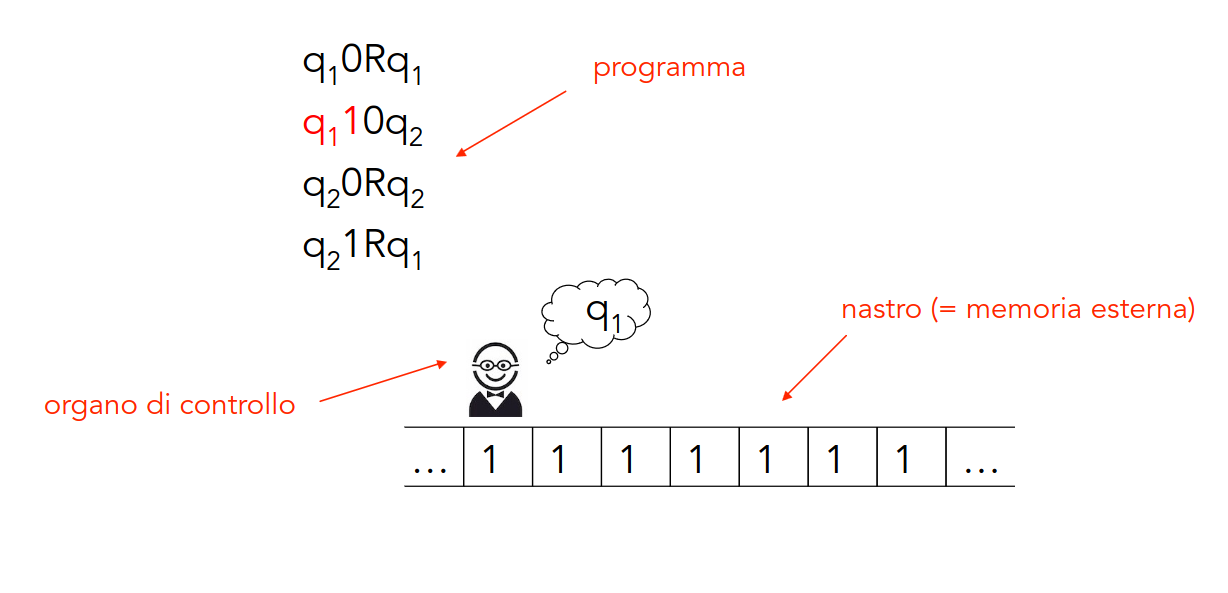
\includegraphics[scale = 0.35]{images/Turing.png}
    \caption{Macchine di Turing come Computer.}
\end{figure}

\dfn{Macchina universale}{
    Una \newfancyglitter{macchina universale} ($U$) è una macchina di Turing
    che può simulare il comportamento di qualsiasi altra macchina di Turing ($M$)
    dato il suo programma ($I_M$) per ogni dato $x$:

    $$U(I_M, x) = M(x)$$

    È possibile che $U$ sia più complessa di $M$. In informatica, il
    programma di $U$ è chiamato \newfancyglitter{interprete}. 

    }

    \nt{Questo risultato suggerirà a von Neumann la possibilità di
    automi che generano automi di pari o maggiore complessità.}


\subsection{Non tutte le funzioni sono calcolabili da una macchina di Turing}

Per dimostare che non tutte le funzioni sono calcolabili da una macchina di Turing  si può
utilizzare la \fancyglitter{diagonalizzazione di Cantor}\footnote{Visto nel corso "Matematica discreta".}:
\begin{itemize}
    \item [$\Rightarrow$] Si immagina di poter numerare le funzioni da $\bbN$ in $\bbN$;
    \item [$\Rightarrow$] Si considera una funzione da $\bbN$ in $\{0,1\}^\bbN$;
    \item [$\Rightarrow$] Questo elenco può essere visto come una tabella;
    \item [$\Rightarrow$] Si vuole dimostrare che esiste una sequenza che non è in questa tabella;
    \item [$\Rightarrow$] Si prende la diagonale, che interseca tutte le righe in un punto;
    \item [$\Rightarrow$] Si cambiano tutti i valori della diagonale (0 diventa 1 e viceversa);
    \item [$\Rightarrow$] La diagonale trasformata può essere una riga dell'originale?
    \item [$\Rightarrow$] No, perchè differisce da ogni riga in almeno un punto.
\end{itemize}

\begin{figure}[h]
    \centering
    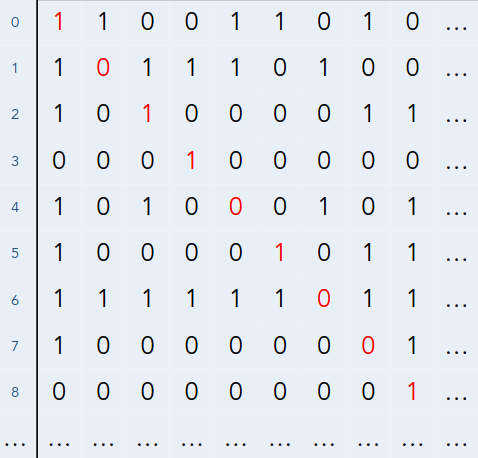
\includegraphics[scale = 0.38]{images/Diagonalizzazione.png}
    \caption{Diagonalizzazione di Cantor.}
\end{figure}

\begin{figure}[h]
    \centering
    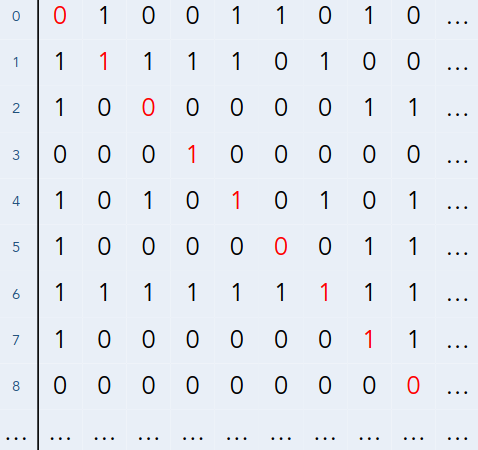
\includegraphics[scale = 0.38]{images/Diagonalizzazione 2.png}
    \caption{Diagonalizzazione di Cantor, inversione della diagonale.}
\end{figure}

\cor{Problemi indecidibili}{
    Non esiste una macchina di Turing $M$ che, operando su un nastro che contiene:
    \begin{itemize}
        \item [$\Rightarrow$] La descrizione di una qualsiasi macchina di Turing $T$;
        \item [$\Rightarrow$] Un input $x$.
    \end{itemize}
    termina sempre i suoi calcoli scrivendo sul nastro il valore $M(T, x)$ dove:
    \begin{itemize}
        \item [$\Rightarrow$] $M(T, x) = 1$ se $T(x)$ termina;
        \item [$\Rightarrow$] $M(T, x) = 0$ se $T(x)$ non termina.
    \end{itemize}
}
\nt{Il problema della fermata è indecidibile.}

\section{Von Neumann: il Computer come Organismo Artificiale}

Von Neumann, matematico e fisico ungherese\footnote{Già visto
nella prima parte del corso.}, fu influenzato dalle idee di
McCulloch e Pitts\footnote{
    \textit{A logical calculus of the ideas immanent in nervous activity}.
}, che avevano definito un modello di neurone
le cui reti potevano essere caratterizzate come \fancyglitter{automi finiti}\footnote{Notato da Kleene nel 1951}.

\begin{figure}[h]
    \centering
    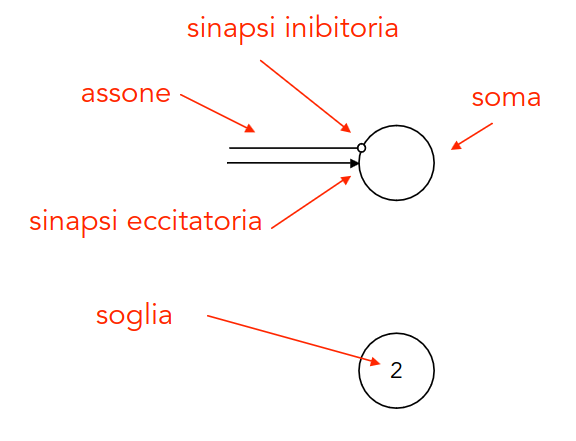
\includegraphics[scale = 0.5]{images/McCulloch-Pitts.png}
    \caption{Il neurone di McCulloch e Pitts.}
\end{figure}

\subsubsection{}

Nel 1945, von Neumann pubblicò il "First Draft of a Report on the EDVAC" in cui
descriveva gli elementi di un calcolatore in termini "biologici" utilizzando
il modello di McCulloch e Pitts:

\begin{itemize}
    \item [$\Rightarrow$] \fancyglitter{CPU}: neuroni di associazione;
    \item [$\Rightarrow$] \fancyglitter{Input}: neuroni sensoriali;
    \item [$\Rightarrow$] \fancyglitter{Output}: neuroni motori.
\end{itemize}

\subsubsection{}

L'obiettivo di von Neumann era quello di \fancyglitter{unificare}, tramite una
teoria generale degli automi, il lavoro di Turing sulle macchine teoriche,
il lavoro di McCulloch e Pitts sui neuroni e il lavoro di Shannon sulla
teoria dell'informazione\footnote{Si vedrà nel prossimo capitolo.}.

\nt{Questo tentativo verrà criticato dai neurofisiologi perché
tentava di descrivere computer e cervello assiomatizzando il comportamento
di \fancyglitter{scatole nere}.}

\subsection{Automi cellulari}

Negli anni '40, a Los Alamos, von Neumann e Ulam ebbero l'idea di
automi che operino su una griglia di celle infinita (bidirezionale).
Ogni cella ha un proprio stato e lo stato di una cella in un'istante $T$
dipende dallo stato delle celle adiacenti in un istante $T - 1$. Il modello
di von Neumann e Ulam aveva 29 stati.

\clm{}{}{
    Da notare che la nozione di \fancyglitter{celle adiacenti} è relativa:
    per von Neumann erano solo 4 (nord, sud, est, ovest), mentre per Moore
    erano 8 (aggiungeva anche le diagonali). Oltre a questo esistono altri modelli con
    celle esagonali e con forme diverse.
}

\begin{figure}[h]
    \centering
    
\includegraphics[scale = 0.3]{images/Automi cellulari.png}
    \caption{Ci sono differenti versioni.}
\end{figure}

\paragraph{Per von Neumann c'erano due modi di descrivere gli automi cellulari:}

\begin{itemize}
    \item [$\Rightarrow$] \fancyglitter{McCulloch-Pitts (modo sintetico)}: strutture
    costruite a partire da elementi più semplici. Bisogna solo definire gli elementi e le loro connessioni (può essere complesso);
    \item [$\Rightarrow$] \fancyglitter{Turing (modo integrale)}: si descrive, tramite assiomi, l'intero automa senza descrivere
    gli elementi da cui è composto, ma solo il loro comportamento.
\end{itemize}

\begin{figure}[h]
    \centering
    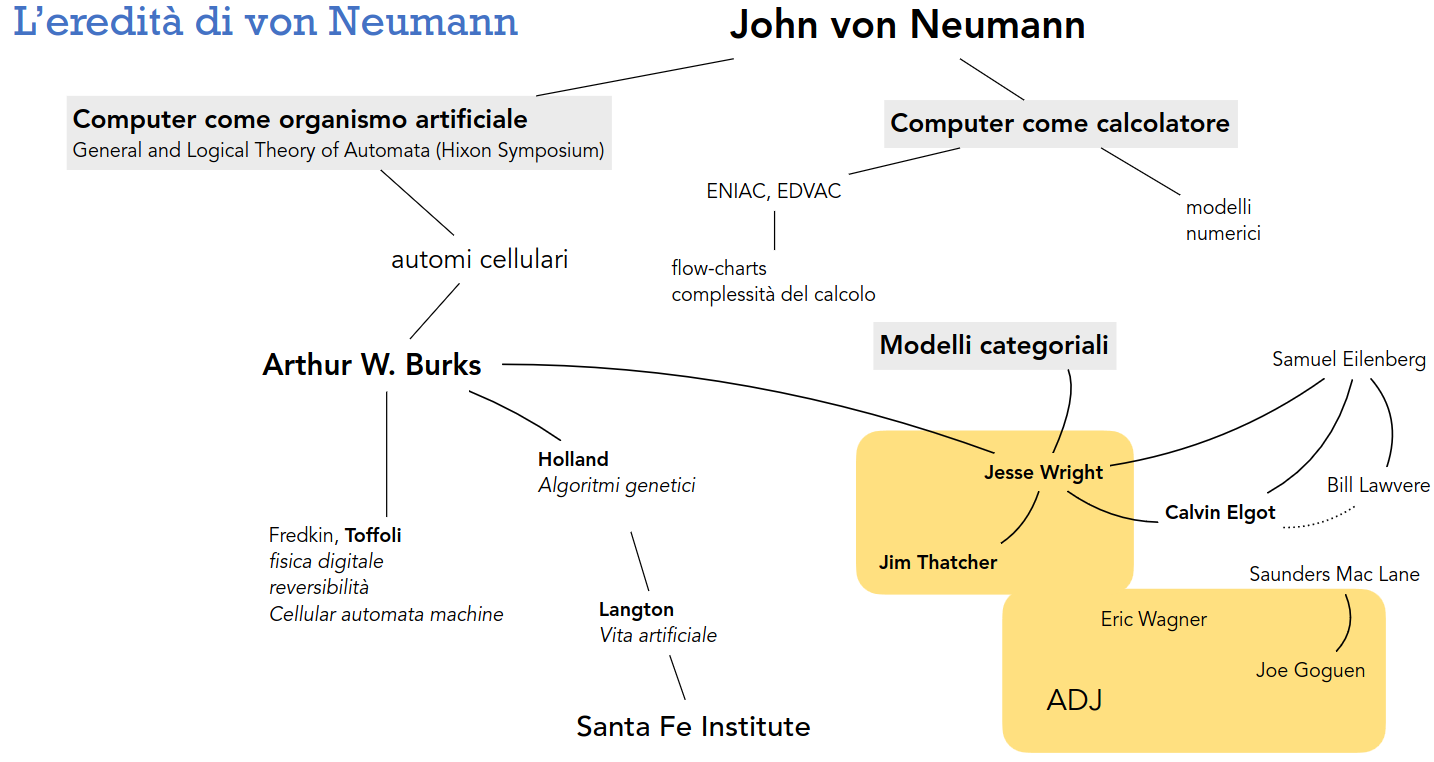
\includegraphics[scale = 0.33]{images/V1.png}
    \caption{Sommario.}
\end{figure}

\subsection{La Vita Artificiale secondo Conway (Game of Life)}

\dfn{Game of Life}{
    Il \newfancyglitter{Game of Life} è un automa cellulare ideato da John Conway nel 1970.
    Si basa su una griglia bidimensionale di celle quadrate, ognuna delle quali può essere
    in uno di due stati: vivo o morto. Le celle comunicano con le otto celle adiacenti.
    È un gioco a zero giocatori, cioè il suo sviluppo è determinato solo dallo stato iniziale.
}

\cor{Regole}{
    Le regole sono le seguenti:
    \begin{itemize}
        \item [$\Rightarrow$] Una cella morta con esattamente tre celle vive adiacenti diventa viva;
        \item [$\Rightarrow$] Una cella viva con due o tre celle vive adiacenti rimane viva;
        \item [$\Rightarrow$] In tutti gli altri casi la cella muore.
    \end{itemize}
}

\begin{figure}[h]
    \centering
    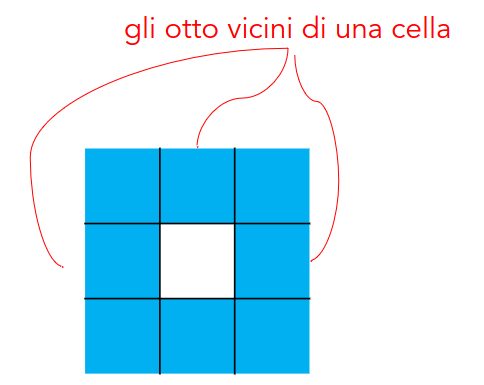
\includegraphics[scale = 0.3]{images/Conway.png}
    \caption{Game of Life.}
\end{figure}

\nt{Una configurazione famosa è il \fancyglitter{glider} (aliante), che si muove
nella griglia.}

\begin{figure}[h]
    \centering
    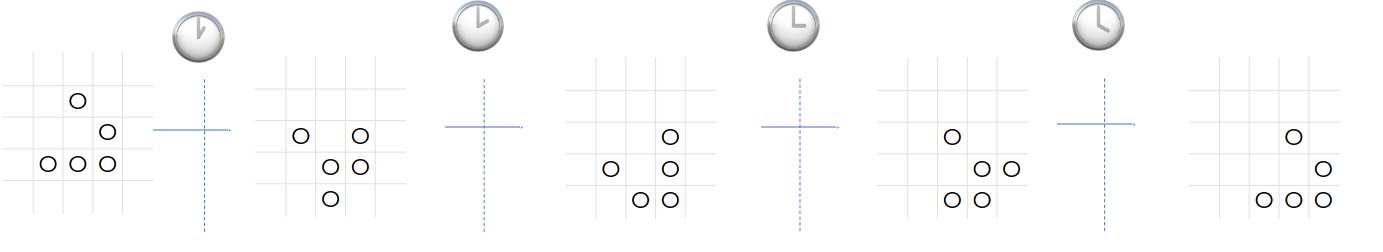
\includegraphics[scale = 0.3]{images/Glider.png}
    \caption{Glider.}
\end{figure}

\definecolor{chaptergrey}{rgb}{0,0,0.7}
\ifnum\layout=2 
    \fancyhf{}      
    \renewcommand{\headrulewidth}{0pt}
    \renewcommand{\chaptermark}[1]{\markboth{#1}{}}

    \fancyhead[LE]{\nouppercase{\textbf{\textcolor{chaptergrey}{\chaptername}}~ \thechapter~ |~ \leftmark}}
    \fancyhead[RO]{\nouppercase{ \rightmark}}
    \fancyfoot[LE,RO]{\thepage}
    \fancypagestyle{plain}{         
    \fancyhf{}
    \fancyfoot[LE,RO]{\thepage}}    
 \else          
    \renewcommand{\headrulewidth}{0pt}
    \fancyhf{}                  
    \fancyhead[C]{\nouppercase{ \leftmark}}
    \fancyfoot[C]{\thepage}
\fi

\chapter{Informazione e cibernetica}

\section{Shannon}

Claude Shannon è un matematico che ha lavorato per la Bell Labs, e ha scritto un articolo nel 1948,
\textit{A Mathematical Theory of Communication}, in cui ha definito la teoria dell'informazione\footnote{Nella laurea magistrale è presente il corso "Teoria dell'Informazione" che approfondice questi argomenti.}: 
"il problema fondamentale della comunicazione è quello di 
riprodurre ad un punto, esattamente o con qualche approssimazione, un messaggio
scelto in un altro punto".

Shannon definisce un contesto tecnico di termini:
\begin{itemize}
    \item [$\Rightarrow$] \fancyglitter{Emittente ricevente}: il mittente è colui che invia il messaggio, il ricevente è colui che lo riceve.
    \item [$\Rightarrow$] \fancyglitter{Messaggio}: è l'informazione che si vuole trasmettere.
    \item [$\Rightarrow$] \fancyglitter{Rumore}: è tutto ciò che può interferire con la trasmissione del messaggio.
    \item [$\Rightarrow$] \fancyglitter{Informazione}: è la quantità di incertezza che si riduce nel ricevente dopo aver ricevuto il messaggio.
\end{itemize}


\nt{L'informazione in  sé è considerata in base al numero di possibili 
messaggi che possono essere inviati.}

\begin{figure}[h]
    \centering
    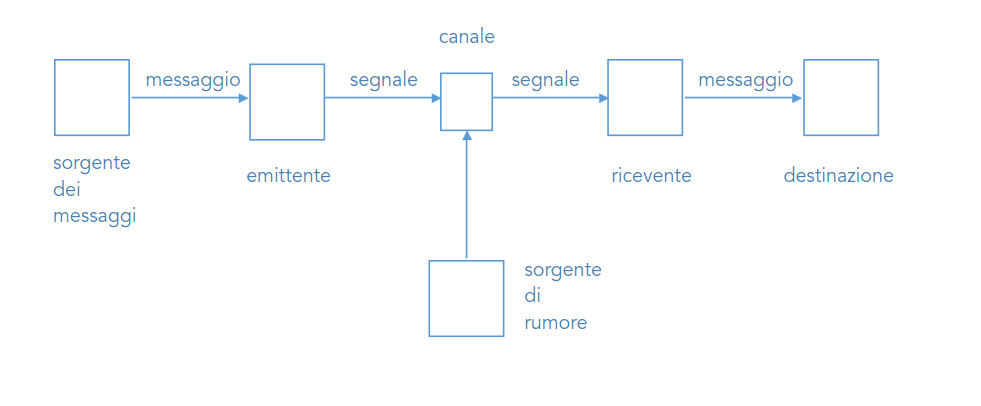
\includegraphics[scale=0.35]{images/Shannon.png}
    \caption{Schema di Shannon}
\end{figure}

\clm{}{}{
    L'informatica non è solamente uno scheletro che può essere riempito con
    qualsiasi cosa. Alla sua base vi sono idee e atteggiamenti fondanti che
    possono essere applicati in molti campi. Un esempio è la cibernetica che ha 
    avuto una breve durata (circa 20 anni), ma ha avuto un impatto molto forte
    su molti campi.

    Esiste un'epistemologia dell'informatica, che ne studia
    le basi e le fondamenta. 
    
    Se si vuole approfondire l'argomento, nella prima parte del corso
    "Metodologie e Tecnologie Didattiche dell'Informatica" (MTDI o PREFIT)
    si ha una panoramica "motivazionale" sulle basi dell'informatica e sul suo
    essere una scienza.    
}

\subsection{Il modello di comunicazione}

Il modello di comunicazione di Shannon purtroppo non mette in evidenza
il fattore temporale e il ritardo. Quando si comunica in un contesto asincrono
bisogna utilizzare un sistema di feedback per capire se il messaggio è stato
ricevuto correttamente\footnote{Per esempio il sistema di ACK (Acknowledgement) di TCP
visto nel corso "Reti I"/"Reti di calcolatori".}. Il modello di comunicazione di Shannon
ha avuto varie interpretazioni, una delle quali è quella di Chapman.

\begin{figure}[h]
    \centering
    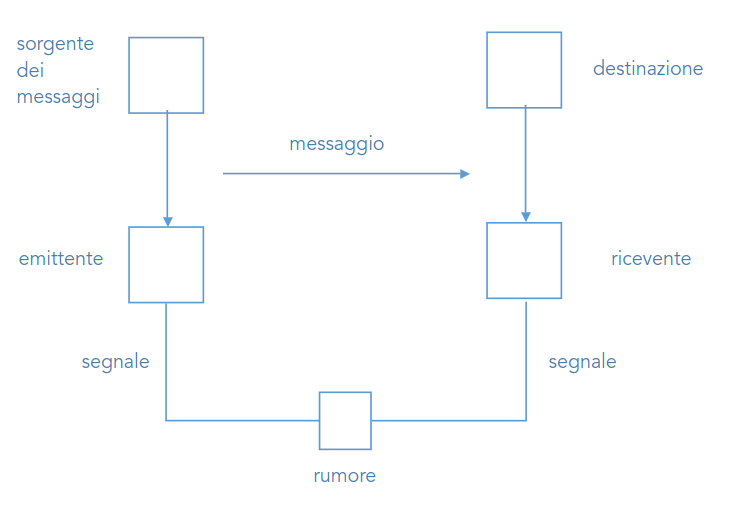
\includegraphics[scale=0.35]{images/Chapman.png}
    \caption{Modello di comunicazione di Shannon, reinterpretato da Chapman.}
\end{figure}
\subsubsection{}
In questa interpretazione vengono identificati i livelli a cui i segnali possono esistere:
\begin{itemize}
    \item [$\Rightarrow$] Nello strato basso è presente il rumore;
    \item [$\Rightarrow$] Al livello superiore è presente il messaggio.
\end{itemize}

\section{Cibernetica e neurofisiologia}

La cibernetica viene codificata da Norbert Wiener nel 1948, e si occupa di studiare i sistemi di controllo e di comunicazione nei sistemi biologici 
e nelle macchine.

Von Neumann aveva come obiettivo l'unificazione del lavoro di McCulloch e Pitts con il lavoro di Shannon e di Turing. Per Wiener,
la nozione unificante era il feedback, mentre per von Neumann era la nozione di automa come
elaboratore di informazione.

\subsubsection{Lavori di von Neumann sugli automi:}

\begin{itemize}
    \item [$\Rightarrow$] \fancyglitter{The general and logical theory of automata}, Hixon Symposium, 1948;
    \item [$\Rightarrow$] \fancyglitter{Theory and organization of complicated automata}, serie di 5 lezioni all'università dello Illinois, 1949;
    \item [$\Rightarrow$] \fancyglitter{Probabilistic logics and the synthesis of reliable organisms from unreliable components}, appunti delle lezioni alla Caltech, 1952;
    \item [$\Rightarrow$] \fancyglitter{The Theory of Automata: Construction, Reproduction, Homogeneity}, 1952-1953;
    \item [$\Rightarrow$] \fancyglitter{The computer and the brain}, Yale University Press, 1956 pubblicato postumo.
\end{itemize}

\subsubsection{}

Per ricapitolare le relazioni tra i vari "attori":

\begin{itemize}
    \item [$\Rightarrow$] \fancyglitter{Shannon - Turing}: si incontrano nel 19343 ai Bell Labs, e discutono di comunicazione\footnote{Da ricordare Enigma e la crittografia.};
    \item [$\Rightarrow$] \fancyglitter{Wiener - Von Neumann - McCulloch - Pitts}: partecipano alle conferenze di Macy la cui nozione centrale è il messaggio (con le accezioni di Shannon);
    \item [$\Rightarrow$] \fancyglitter{Wiener - McCulloch - Pitts}: membri del RLE;
    \item [$\Rightarrow$] \fancyglitter{Von Neumann - Turing}: si incontrano nel 1937 a Princeton. Nel 1939 von Neumann offre a Turing un posto di lavoro come assistente a Princeton, ma Turing rifiuta;
    \item [$\Rightarrow$] \fancyglitter{Shannon - Wiener}: sviluppano una teoria matematica e della comunicazione basata sulla concezione dell'informazione/entropia di un insieme di messaggi.
\end{itemize}

\clm{}{}{Pare che Shannon adorasse il monociclo e che spesso tenesse dei party
in cui si esibiva in numeri di equilibrismo.
}

\begin{figure}[h]
    \centering
    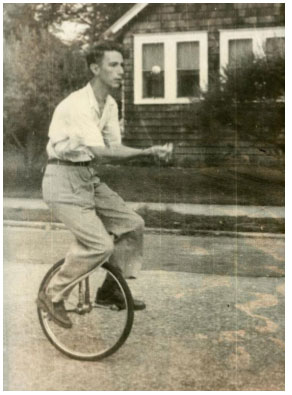
\includegraphics[scale=0.35]{images/Shannon monocycle.jpg}
    \caption{Shannon sul monociclo}
\end{figure}

\section{Von Neumann e la termodinamica del calcolo}

Von Neumann cercò di valutare il costo energetico minimo per un
atto elementare di generazione di informazioni. Da ciò deriva, nel 1949,
la formula:

$$kT \log_e N$$

\begin{itemize}
    \item [$\Rightarrow$] $k$: costante di Boltzmann;
    \item [$\Rightarrow$] $T$: temperatura;
    \item [$\Rightarrow$] $N$: numero di alternative o possibili stati.
\end{itemize}

Questo calcolo attira le attenzioni di \fancyglitter{Landauer}, un fisico teorico, 
che non riesce a dimostrarlo, ma osservo che le operazioni logicamente
irreversibili (come l'operazione di cancellazione di un bit) generano entropia
pari alla quantità di informazione cancellata. \fancyglitter{Bennet}, un suo studente,
nel 1973, dimostra che ogni calcolo può essere reso logicamente reversibile.
\fancyglitter{Fredkin} lavora a una base fisica per i calcoli reversibili.

\nt{Da questo tipo di interessi nasce la computazione quantistica (
    che cosa succede se si considera la computazione come composta da operazioni
    maccaniche?).}

\begin{figure}[h]
    \centering
    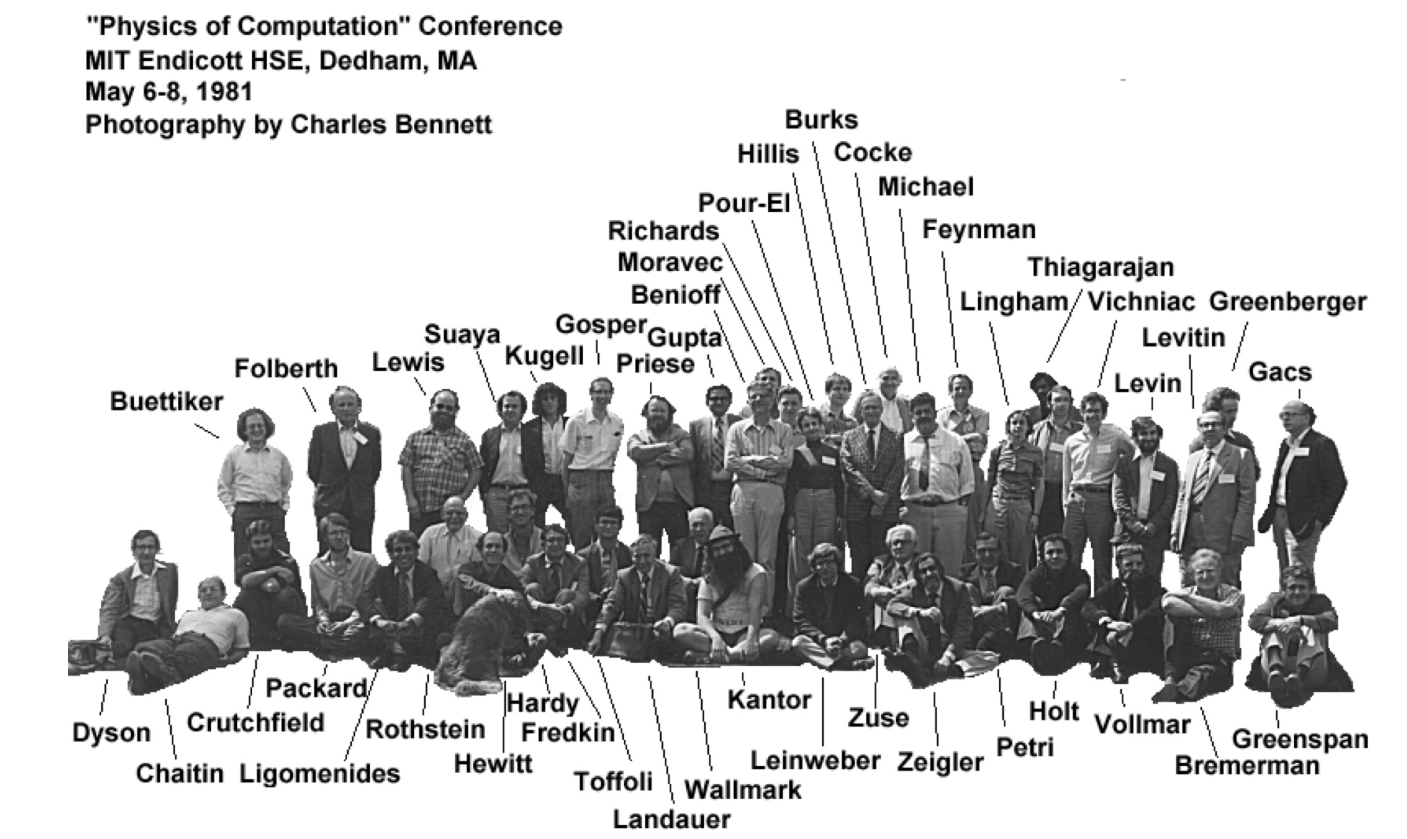
\includegraphics[scale=0.3]{images/Comp.png}
    \caption{Physics of Computation}
\end{figure}

\clm{}{}{
    \begin{itemize}
        \item [$\Rightarrow$] \fancyglitter{Bennet}: è un fisico teorico, non è direttamente
        presente nella foto perchè fu lui a scattarla;
        \item [$\Rightarrow$] \fancyglitter{Landauer}: è presente nella foto in primo piano;
        \item [$\Rightarrow$] \fancyglitter{Fredkin}: è presente nella foto, vicino a Landauer e Toffoli;
        \item  [$\Rightarrow$] \fancyglitter{Toffoli}: fu uno studioso di fisica della computazione che interagi con
        Burks;
        \item  [$\Rightarrow$] \fancyglitter{Burks}: in secondo piano;
        \item [$\Rightarrow$] \fancyglitter{Feynman}, \fancyglitter{Dysan} e altri fisici famosi;
        \item [$\Rightarrow$] \fancyglitter{Zuse}: già visto nella prima parte del corso, inventore dello Z1;
        \item [$\Rightarrow$] \fancyglitter{Kantor}: inventore e specialista dell'informazione come principio ontologico;
        \item [$\Rightarrow$] \fancyglitter{Holt}: esperto di cibernetica;
        \item [$\Rightarrow$] \fancyglitter{Gosper}: inventore della configurazione ad aliante, uno dei primi "hacker".
    \end{itemize}
}

\section{La cibernetica}

Quando si \fancyglitter{comunica} con un'altra persona gli si trasmette un
messaggio, e quando l'altra persona risponde, si riceve un messaggio che contiene
informazioni accessibili a sé stessi e all'altro. Quando si \fancyglitter{controllano}
le azioni di un'altra persona gli si comunica un messaggio (in forma imperativa). 
Tutto ciò si riduce a uno \fancyglitter{scambio di messaggi}.

\dfn{Cibernetica}{
    La \newfancyglitter{cibernetica} può essere vista come una teoria della
    trasmissione dei messaggi e delle sue condizioni che presentano un successo.
}

\nt{Il computer diventa un oggetto cibernetico, in quanto è inserito in un
contesto di comunicazione con esseri umani o con altri computer.}

\subsection{Il feedback e il flusso di messaggi nei sistemi}

Wiener confrontava l'attività umana con quella di figure che danzano sopra
un carillon secondo un modello. Tuttavia il modello in esame è un modello
predisposto in cui il loro passato non ha influenza sul loro futuro. Non 
c'è feedback.

\begin{figure}[h]
    \centering
    
\includegraphics[scale=0.35]{images/IO.png}
    \caption{Modello IO}
\end{figure}

\subsubsection{}

Holt propose l'idea che quando una persona scrive su una macchina premendo il tasto
esso fornisce un feedback tornando indietro. La temporizzazione dei tasti è
ciò che consente la scrittura.
Questo si può estendere all'utente e all'interfaccia: la scelta di un'interfaccia comporta
la progettazione dell'utente indicando cosa si può o non si può fare.

\ex{Scatola nera}{
    Si immagini una scatola con dei pulsanti che si possono premere. Quando si preme un pulsante
    si accende una luce. Prima di poter schiacciare un altro pulsante bisogna controllare che la luce
    si sia accesa. In questo caso la luce è il feedback.
    \begin{center}
        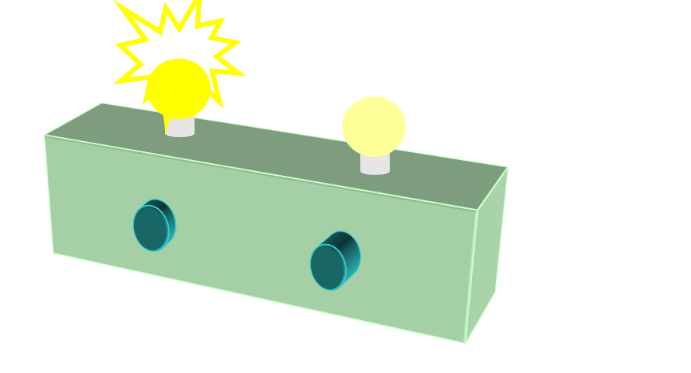
\includegraphics[scale=0.5]{images/Scatola nera.png}
    \end{center}

    Se i pulsanti sono premuti da un operatore che non può vedere le luci e 
    le luci sono visibili a un altro operatore che non può premere i pulsanti,
    non si potrebbe stabilire una connessione tra luci e pulsanti e dunque la connessione non ha 
    succeso.

    \begin{center}
        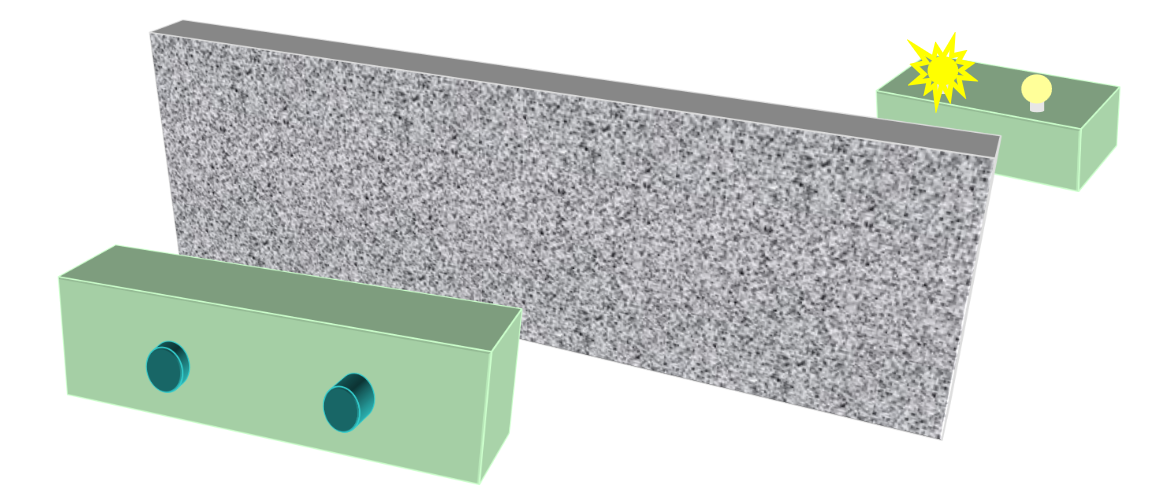
\includegraphics[scale=0.35]{images/Scatola nera 2.png}
    \end{center}

}

\subsection{Osservatori}

In alcuni sistemi, per esempio un termostato, è l'osservatore a concettualizzarlo.
Nei sistemi di secondo ordine, l'osservatore è esso stesso parte del sistema osservato.

\begin{figure}[h]
    \centering
    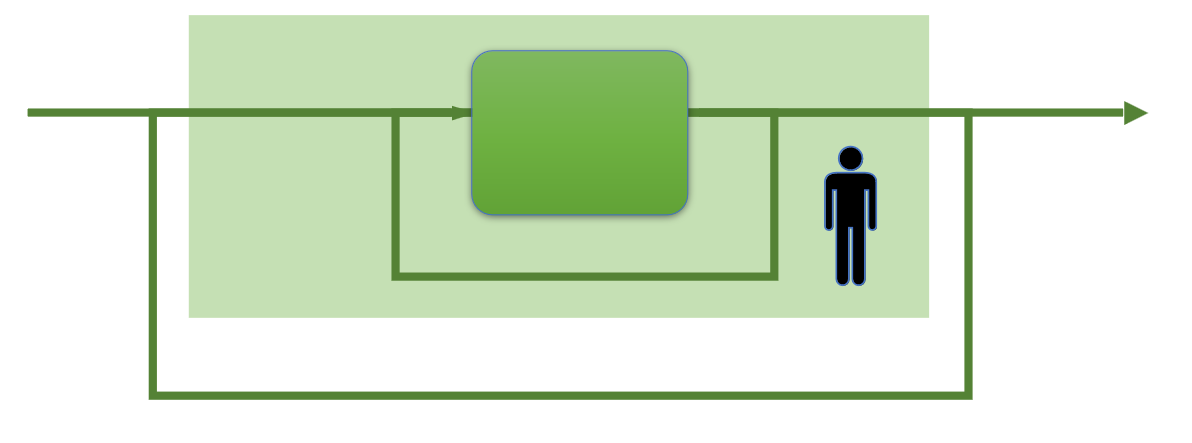
\includegraphics[scale=0.25]{images/Osservatore.png}
    \caption{Osservatore}
\end{figure}

\subsection{Comunicazione sincrona e asincrona}

\dfn{Comunicazione sincrona}{
    La \newfancyglitter{comunicazione sincrona} è una comunicazione in cui il mittente e il ricevente
    sono sincronizzati. 
    
    In una comunicazione sincrona è presente un unico sistema di riferimento
    temporale condiviso da tutti i partecipanti. 

}

\ex{Comunicazione sincrona}{
    \begin{itemize}
        \item [$\Rightarrow$] Chiamata telefonica;
        \item [$\Rightarrow$] Conversazione faccia a faccia;
        \item [$\Rightarrow$] Sistema di posta elettronica in cui i messaggi impiegano $n$ secondi per 
        essere consegnati;
        \item [$\Rightarrow$] Segnali di fumo.
    \end{itemize}
}

\dfn{Comunicazione asincrona}{
    La \newfancyglitter{comunicazione asincrona} è una comunicazione in cui il mittente e il ricevente
    non sono sincronizzati. 
    
    In una comunicazione asincrona non è presente un unico sistema di riferimento
    temporale condiviso da tutti i partecipanti. 

}

\ex{Comunicazione asincrona}{
    \begin{itemize}
        \item [$\Rightarrow$] Sistema di posta elettronica con garanzia di consegna entro $n$ secondi;
        \item [$\Rightarrow$] Sistema postale ordinario;
        \item [$\Rightarrow$] Messaggi in bottiglia.
    \end{itemize}
}

\nt{Nella comunicazione asincrona è necessario un sistema di feedback per capire se il messaggio è stato ricevuto.}

\subsection{Circuiti asincroni}

\dfn{Circuiti asincroni}{
    I \newfancyglitter{circuiti asincroni} sono circuiti in cui i segnali di controllo
    non sono sincronizzati con un segnale di clock (orologio globale).
}

\cor{C-Muller}{
    Un elemento asincrono è il C-Muller per cui l'uscita è 1 se e solo se
    entrambi gli ingressi sono 1 e diventa 0 se entrambi gli ingressi sono 0.
}

\begin{figure}[h]
    \centering
    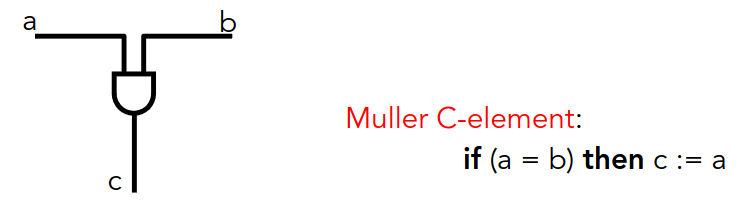
\includegraphics[scale=0.35]{images/C-Muller.png}
    \caption{C-Muller}  
\end{figure}

\nt{Combinando più C-Muller si può costruire un circuito asincrono che implementa
le micropipeline.}

\begin{figure}[h]
    \centering
    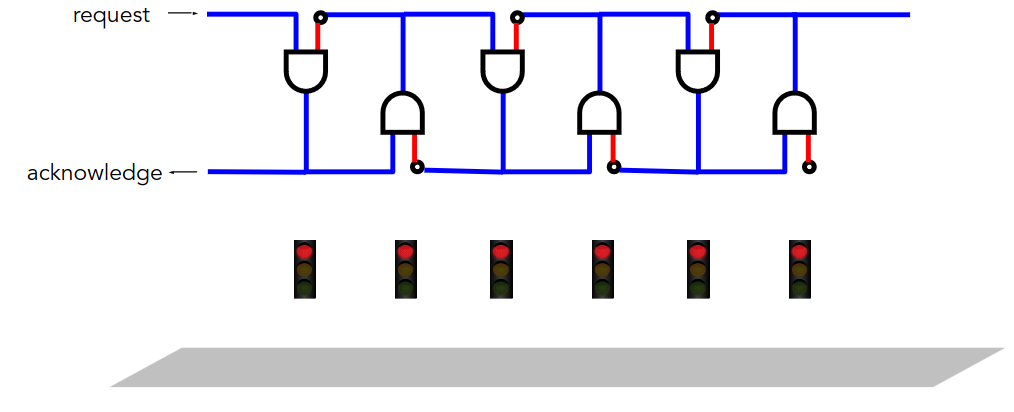
\includegraphics[scale=0.35]{images/Micropipeline.png}
    \caption{Micropipeline}
\end{figure}

\cor{Reti di Petri}{
    Grafi che generalizzano gli automi a stati finiti (DFA e NFA).
    Si hanno posti (condizioni) e transizioni (eventi).
}

\begin{figure}[h]
    \centering
    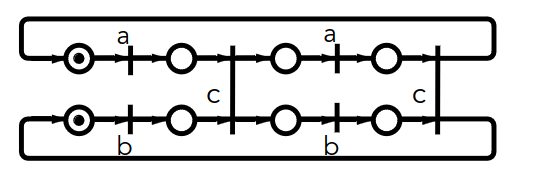
\includegraphics[scale=0.35]{images/Petri.png}
    \caption{Rete di Petri}
\end{figure}












\definecolor{chaptergrey}{rgb}{1,0.75,0}
\ifnum\layout=2 
    \fancyhf{}      
    \renewcommand{\headrulewidth}{0pt}
    \renewcommand{\chaptermark}[1]{\markboth{#1}{}}

    \fancyhead[LE]{\nouppercase{\textbf{\textcolor{chaptergrey}{\chaptername}}~ \thechapter~ |~ \leftmark}}
    \fancyhead[RO]{\nouppercase{ \rightmark}}
    \fancyfoot[LE,RO]{\thepage}
    \fancypagestyle{plain}{         
    \fancyhf{}
    \fancyfoot[LE,RO]{\thepage}}    
 \else          
    \renewcommand{\headrulewidth}{0pt}
    \fancyhf{}                  
    \fancyhead[C]{\nouppercase{ \leftmark}}
    \fancyfoot[C]{\thepage}
\fi
\definecolor{chaptergrey}{rgb}{1,0.75,0.8}
\ifnum\layout=2 
    \fancyhf{}      
    \renewcommand{\headrulewidth}{0pt}
    \renewcommand{\chaptermark}[1]{\markboth{#1}{}}

    \fancyhead[LE]{\nouppercase{\textbf{\textcolor{chaptergrey}{\chaptername}}~ \thechapter~ |~ \leftmark}}
    \fancyhead[RO]{\nouppercase{ \rightmark}}
    \fancyfoot[LE,RO]{\thepage}
    \fancypagestyle{plain}{         
    \fancyhf{}
    \fancyfoot[LE,RO]{\thepage}}    
 \else          
    \renewcommand{\headrulewidth}{0pt}
    \fancyhf{}                  
    \fancyhead[C]{\nouppercase{ \leftmark}}
    \fancyfoot[C]{\thepage}
\fi
\definecolor{chaptergrey}{rgb}{0,0.13, 0.38}
\ifnum\layout=2 
    \fancyhf{}      
    \renewcommand{\headrulewidth}{0pt}
    \renewcommand{\chaptermark}[1]{\markboth{#1}{}}

    \fancyhead[LE]{\nouppercase{\textbf{\textcolor{chaptergrey}{\chaptername}}~ \thechapter~ |~ \leftmark}}
    \fancyhead[RO]{\nouppercase{ \rightmark}}
    \fancyfoot[LE,RO]{\thepage}
    \fancypagestyle{plain}{         
    \fancyhf{}
    \fancyfoot[LE,RO]{\thepage}}    
 \else          
    \renewcommand{\headrulewidth}{0pt}
    \fancyhf{}                  
    \fancyhead[C]{\nouppercase{ \leftmark}}
    \fancyfoot[C]{\thepage}
\fi

\definecolor{chaptergrey}{rgb}{0.21,0.37,0.23}
\ifnum\layout=2 
    \fancyhf{}      
    \renewcommand{\headrulewidth}{0pt}
    \renewcommand{\chaptermark}[1]{\markboth{#1}{}}

    \fancyhead[LE]{\nouppercase{\textbf{\textcolor{chaptergrey}{\chaptername}}~ \thechapter~ |~ \leftmark}}
    \fancyhead[RO]{\nouppercase{ \rightmark}}
    \fancyfoot[LE,RO]{\thepage}
    \fancypagestyle{plain}{         
    \fancyhf{}
    \fancyfoot[LE,RO]{\thepage}}    
 \else          
    \renewcommand{\headrulewidth}{0pt}
    \fancyhf{}                  
    \fancyhead[C]{\nouppercase{ \leftmark}}
    \fancyfoot[C]{\thepage}
\fi


\definecolor{chaptergrey}{rgb}{0.5,0.5,0.5}

\ifnum\layout=2 
    \fancyhf{}      
    \renewcommand{\headrulewidth}{0pt}
    \renewcommand{\chaptermark}[1]{\markboth{#1}{}}

    \fancyhead[LE]{\nouppercase{\textbf{\textcolor{chaptergrey}{\chaptername}}~ \thechapter~ |~ \leftmark}}
    \fancyhead[RO]{\nouppercase{ \rightmark}}
    \fancyfoot[LE,RO]{\thepage}
    \fancypagestyle{plain}{         
    \fancyhf{}
    \fancyfoot[LE,RO]{\thepage}}    
 \else          
    \renewcommand{\headrulewidth}{0pt}
    \fancyhf{}                  
    \fancyhead[C]{\nouppercase{ \leftmark}}
    \fancyfoot[C]{\thepage}
\fi


\end{document}